% !TEX root = main2.tex
% Revision: Gaussian-front existence, proof, and extreme-settlement qualification.
% External project dependencies retained: sec_factor_figures.tex, sec_pipeline.tex, refs.bib.
% The pasted Markdown/HTML escaping has been normalized to LaTeX.
\documentclass[11pt]{article}
\usepackage[margin=1.1in]{geometry}
\usepackage{amsmath,amssymb,amsthm,mathtools}
\usepackage[T1]{fontenc}
\usepackage{microtype}
\usepackage{lmodern}
\usepackage{booktabs}
\usepackage{graphicx}
\usepackage{adjustbox}
\usepackage{float}
\usepackage{xcolor}
\usepackage{enumitem}
\usepackage{needspace}
\setlength{\emergencystretch}{2em}
\usepackage[colorlinks=true,linkcolor=black,citecolor=black,urlcolor=black]{hyperref}
\hypersetup{pdftitle={Generative Risk-Neutral Option Market Models},pdfauthor={Magnus Wiese; Hans Buehler; Blanka Horvath}}

\newcommand{\R}{\mathbb R}
\newcommand{\E}{\mathbb E}
\newcommand{\Q}{\mathbb Q}
\newcommand{\PP}{\mathbb P}
\newcommand{\dd}{\mathrm d}
\newcommand{\dlv}{\Sigma}
\newcommand{\abs}[1]{\lvert #1\rvert}
\newcommand{\ip}[2]{\langle #1,#2\rangle}
\newcommand{\one}{\mathbf 1}
\newcommand{\Var}{\operatorname{Var}}
\newcommand{\Gh}{\widehat G}
\newcommand{\Nh}{\widehat N}
\newcommand{\removeblock}[1]{}

\theoremstyle{plain}
\newtheorem{theorem}{Theorem}[section]
\newtheorem{proposition}[theorem]{Proposition}
\newtheorem{lemma}[theorem]{Lemma}
\newtheorem{corollary}[theorem]{Corollary}
\theoremstyle{definition}
\newtheorem{assumption}[theorem]{Assumption}
\theoremstyle{remark}
\newtheorem{remark}[theorem]{Remark}

\title{\textbf{Generative Risk-Neutral Option Market Models}}

\author{Magnus Wiese$^{*}$\qquad Hans Buehler$^{*}$\qquad Blanka Horvath$^{*,\#}$\\[0.6em]
{\small $^{*}$Mathematical Institute, University of Oxford, 
$^{\#}$Oxford-Man Institute, University of Oxford}}
\date{\today}

\begin{document}
\maketitle

\begin{abstract}
We present a European option market model with smooth strike interpolation, based on the SANOS~\cite{SANOS2026} framework.
Under explicit local regularity and a square-integrable vol-of-vol envelope, we prove existence
of its risk-neutral density and price processes at the fixed model expiries. The discrete
backbone is absorbed at extreme strikes; finite positive DLV coordinates extend through
every interior settlement, but are not required at an absorbing endpoint.

In spirit,
it is a stocastic model for local volatility when the latter is used as a representation of a European option price surface, not as a pricing model.

We illustrate the strength of our approach on S\&P Index Option data from January 2022 to August 2025.
We show that the model's initial state fits within bid/ask for more than 95\% of relevant market option prices.\footnote{
The model presented was trained for daily expiries up to 25 business days and strikes between $[\exp(-2.5 \sigma_{atm} \sqrt{t}), \exp(+1.5 \sigma_{atm} \sqrt{t})]$.}
We then train the model dynamics under~$\PP$ and~$\Q$ and show that the model is indeed free of arbitrage
while fitting the dynamics of the market well.
\end{abstract}

\tableofcontents

\section{Introduction}\label{sec:intro}

This article presents an arbitrage-free market model for for smooth surfaces of European option prices. While not strictly the first of is kind,
it is the first model with an industy-grade ability to fit the current market, allow for smooth interpolation of the entire option surface at each time,
and provide an explicit construction of the continuous time risk-neutral drift for both (discrete local) volatilities and spot. It also has a natural
estimation strategy for its parameter space.

The core architecture follows the SANOS approach~\cite{SANOS2026} which models the stock price as the product
of a time-and-state discrete process~$X$ and a smoothing process~$Y$, in our case Black~\&~Scholes.
The former is used to encode the option market using a discrete form of local volatilities as code book. That does not mean
that the model is a local volatility model -- we merely use the implied local volatilities as a convenient representation of the option surface.
Compared to using implied volatilities the advantage is that mere positivity of the local volatilities is sufficient to ensure
the the option market is free of static arbitrage at all times. We have shown in~\cite{SANOS2026} that this representation
can be fitted to real life market data very efficiently using linear programming.

The key
contribution in this paper is showing how to construct a dynamic model of SANOS option call prices which are not only statically but
also dynamically free of arbitrage. We show the theoretical construction of the corresponding risk-neutral measure~$\mathbb{Q}$
and prove existence of the respective martingale processes at the model expiries in Theorem~\ref{thm:existence},
with the extreme-settlement convention specified there. We then discuss implementation
and estimate our model on S\&P Index Option data from January 2022 to August 2025. We fit our daily model parameters to observed bid/ask prices and then proceed to
estimate both $\Q$ and its drift under $\PP$. We show that
on this data set more than 90\% of calibrated
model prices fit within observed market bid/ask spreads even with the simplistic grid architecture we present here.

We then show that model dynamics under the risk-neutral indeed have numerically zero conditional and unconditional drift. We test this first
with a restricted universe of 570 tradable instruments in a number of different set ups. We then also show that even using all 5001 instruments
the risk-neutrality is preserved. Ours is the first model being able to show such a result for a number of instruments which far exceeds
the number of driving stochastic factors.

The model presented here is distinct from our own DYSANOS~\cite{DYSANOS2026}. There, we focused on learning
realistic market dynamics for smooth statically arbitrage-free SANOS
surfaces under~$\PP$.
We did also construct an equivalent risk-neutral measure~$\Q$ numerically using the \emph{martingale measure} approach introduced in~\cite{removedrift}.
While this method is model-free and can in theory be applied to any option market model under~$\PP$, it is numerically heavy and in practise
restricted to making only a fairly limited number of the overall tradable instruments
dynamically arbitrage-free.\footnote{In~\cite{DYSANOS2026} we used 49 instruments per simulated date.} In the current work we cover all options with
an explicit construction of the risk-neutral drift at the model expiries, which is far more efficient than the numerical martingale measure approach.

\subsubsection*{Related Work}

Our approach most closely related to the seminal but unpublished work~\cite{Wissel2007}
which extends their earlier works~\cite{SchweizerWissel2008} and~\cite{Schweizer2007}. From a
theoretical perspective, our approach is a version of~\cite{CarmonaNadtochiy2008} where
the authors derive related risk-neutral drift conditions for continuous time local volatility models, 
but without a tangible implementation strategy. Our results
can be seen as a joint extension of the two papers, plus  smoothing and market-fit from our SANOS~\cite{SANOS2026}. 

In~\cite{TANGET} the 
authors solve the problem of finding a dynamically arbitrage-free evolution of the full option surface via products of indepdent Levy processes. While structurally
very elegant, option prices generated by products of independent increment processes do not typically fit well to equity index European option surfaces. 
Our approach also has the advantage of being numerically accessible.
In particular, our model prices can be fit very efficiently within nearly all\footnote{In below experiments, above 90\%.} of observed market bid/ask prices
using the  linear programming SANOS~\cite{SANOS2026} calibration method.

There are a number of works on generative equity option market dynamics -- not least our
own~2019 work \cite{WieseEtAl2019OptionMarkets} and the multi-asset version~\cite{WieseEtAl2021MultiAsset} -- which simulate
discrete strictly arbitrage-free option surfaces. However, most other approaches
are not strictly free of arbitrage and do not have analytical corresponding risk-neutral dynamics.
To address the absence of an analytical risk-neutral measure, we presented in~ \cite{removedrift} 
a model-free approach
to learning such measure. However,  that method is numerically challenging
for large number of tradable options as discussed in~\cite{DYSANOS2026}.

For interest rate option markets the reference model in the same class is the BGM Model~\cite{BGM}.

\section{Stochastic Smooth Discrete Local Volatility}

In this section we introduce the core model architecture for our \emph{Stochastic 
Smooth Discrete Local Volatility model}.
We follow the core SANOS~\cite{SANOS2026} idea of writing our equity process $S$ as product
\begin{equation}
\label{eq:S} 
S_t = X_t Y_t 
\end{equation}
of a \emph{Stochastic Discrete Local Volatility (SDLV)} process $X$ which is used to fit to current market condition and 
whose state parameters will have consistent $\PP$ and $\Q$ dynamics, and an independent\footnote{Under both $\PP$ and $\Q$.} and rather trivial smoothing process $Y$ whose dynamics under $\PP$ and $\Q$ are the same.

The process $Y$ will just be a Black~\&~Scholes process with fixed volatility~5\%. Given observed bid/ask market data it was shown in~\cite{SANOS2026} how to fit
a discrete local volatility surface in the presence of such process. 

In the remainder of this section we focus on the SDLV process itself.

\subsection{Stochastic Discrete Local Volatility (SDLV)}

Our \emph{Stochastic Discrete Local Volatility (SDLV)} risk-neutral model will be defined on a \emph{fixed} expiry and cash strike grid. It will not use a floating grid in its option market dynamics.\footnote{This is not to be confused to 
how the model parameters are estimated using historic market data. We explain estimation section~\ref{sec:estimation}.} We will use ``$t$'' to refer to 
model time. Denote initial spot by~$X_0>0$.

For now let $0=T_0<T_1<\dots<T_M$ be the fixed model expiry dates, and assume that $K_0<K_1<\cdots<X_0<\cdots<K_{N+1}$ are the fixed model cash strikes, where 
$K^0$ and $K^{N+1}$
are boundary strikes which are far away from the inner strikes, c.f.~\cite{SANOS2026}.\footnote{In our experiments the inner strikes are given as range of strikes
in from $K^1=\exp(-2.5 \sigma_{atm}(T_M) \sqrt{T_M})$ to $K^N=\exp(+1.5 \sigma_{atm}(T_M) \sqrt{T_M})$ with boundaries set to $K^0=K^1/2$ and $K^{N+1}=3 K^N / 2$; see
section~\ref{sec:numerics} for specifics.
}

Assume that $t$ is the current model time and let $T_k$ be the front expiry such that $T_{k-1}\leq t<T_k$.
Our model is given at any time~$t$
by the current spot $X_t$ and future densities $q_t^j$, where $q_t^{j,i}$ represents the risk-neutral density of the $i$-th cash strike at future expiry $T_j$.

Such discrete densities have been shown in~\cite{BuehlerRyskin2016} to admit an equivalent representation via (squared) \emph{discrete local volatilities} $\Sigma_t^{j,1},\ldots,\Sigma_t^{j,N}$ in the following form:
there is a tridiagonal matrix~$\Omega_j$\footnote{
Densities are column vectors, so $\Omega_j$ is the forward operator.
For $i=1,\ldots,N$, set
\[
 \gamma_i^{j,\pm}:=
 \frac{\pm(K^i)^2(T_j-T_{j-1})}
 {(K^{i+1}-K^{i-1})(K^{i\pm1}-K^i)}>0.
\]
Its only nonzero entries in interior column $i$ are
\[
 (\Omega_j)_{i-1,i}=\gamma_i^{j,-},\quad
 (\Omega_j)_{i,i}=-(\gamma_i^{j,-}+\gamma_i^{j,+}),\quad
 (\Omega_j)_{i+1,i}=\gamma_i^{j,+}.
\]
Both boundary columns vanish. In particular,
$\one^\top\Omega_j=K^\top\Omega_j=0$; see~\cite{SANOS2026}.
} for each $j>k$ such that 
\begin{equation}
q_t^{j-1}=M_t^jq_t^j \ ,
\qquad
M_t^j:=I-\Omega_jS_t^j \ ,
\qquad
S_t^j:=\operatorname{diag}(0,\Sigma_t^{j,1},\ldots,
\Sigma_t^{j,N},0) 
\label{eq:hb_dlv}
\end{equation}
where $M^j_t$ is an invertible tridiagonal M-matrix for every non-negative $S_t^j$.
Given the front density and the non-negative DLV surface, the recursion uniquely determines
probability densities with the same first moment. Their martingale property under the
specified dynamics, and existence through expiry, are proved in Section~\ref{sec:existence}.

\subsection{Risk-Neutral Dynamics}

Under a risk-neutral measure~$\Q$ densities are martingales. We will now turn this property into conditions on dynamics of the (squared) discete local volatilities, and, 
jointly the front density and spot. 
Our approach follows in spirit that of~\cite{Wissel2007} in the sense that we rely on the martingale property of a discrete set of tradable derivative assets.
However, we reframe it in a much more accessible coordinate system.

Assume that $W$ is a $d$-dimensional Brownian motion. We designate $W^1$ as the
spot factor: spot is always driven by $dW_t^1$.

\subsubsection{Future Densities}
\label{sec:future-densities}

Each density coordinate
is a martingale. We therefore specify the front-density diffusion as
\[
dq_t^k=E_t^{k;1}\,dW_t^1 \ ,
\qquad
E_t^{k;1}:=\operatorname{diag}(q_t^k)\eta_t^{k;1} \ ,
\qquad E_t^{k;f}:=0\quad(f=2,\ldots,d),
\]
where $E_t^{k;1}\in\mathbb R^{N+2}$ must satisfy
$\one^{\!\top}E_t^{k;1}=0$, so that $q_t^k$ retains unit mass. The
remaining Brownian factors do not directly move the front density. They
drive the stochastic DLV surface, while $\xi_t^{j,\cdot,1}$ determines its loading on the spot factor.
Future density volatilities $\eta_t^j$ for $j>k$ will be obtained recursively.

For future expiries $T_j$ with $j>k$, assume the discrete local volatity squared is given as
\[
\frac{ d\Sigma_t^{j} }{ \Sigma_t^{j} }
= \mu^j_t\,dt
+ \xi^j_t\,dW_t,
\]
where $\xi_t^j\in\mathbb R^{N\times d}$ is given and
$\mu_t^j\in\mathbb R^N$ is the unknown risk-neutral drift. We write this as
\[
dS_t^j=A_t^j\,dt+\sum_{f=1}^dB_t^{j;f}\,dW_t^f,
\]
with
$A_t^j
:=\operatorname{diag}(0,\Sigma_t^{j,1}\mu_t^{j,1},\ldots,
\Sigma_t^{j,N}\mu_t^{j,N},0)$ and $B_t^{j;f}
:=\operatorname{diag}(0,\Sigma_t^{j,1}\xi_t^{j,1;f},\ldots,
\Sigma_t^{j,N}\xi_t^{j,N;f},0).$
With the above
\[
dM_t^j=-\Omega_j\,dS_t^j
=-\Omega_jA_t^j\,dt
-\sum_{f=1}^d\Omega_jB_t^{j;f}\,dW_t^f.
\]
Setting $dq_t^j=\sum_fE_t^{j;f}\,dW_t^f$ for an unknown $E_t^{j;f}$ yields
\begin{eqnarray}
dq_t^{j-1}
& = & M_t^j\,dq_t^j+(dM_t^j)q_t^j+d[M^j,q^j]_t\\
& = & \sum_{f=1}^d
\left(M_t^jE_t^{j;f}-\Omega_jB_t^{j;f}q_t^j\right)dW_t^f
-\Omega_j\left(A_t^jq_t^j
+\sum_{f=1}^dB_t^{j;f}E_t^{j;f}\right)dt \ .
\end{eqnarray}
Matching the diffusion coefficients gives
\begin{equation}
\label{eq:vol_hb}
E_t^{j;f}
=(M_t^j)^{-1}
\left(E_t^{j-1;f}+\Omega_jB_t^{j;f}q_t^j\right)
\in\mathbb R^{N+2} \ \ \ \mbox{and} \ \ \ \eta_t^{j,i;f}=\frac{ E_t^{j,i;f} }{ q_t^{j,i} } \ .
\end{equation}
The drift must vanish, hence
\[
\Omega_j\left(A_t^jq_t^j
+\sum_{f=1}^dB_t^{j;f}E_t^{j;f}\right)=0.
\]
The restriction of $\Omega_j$ to vectors supported on the interior nodes
is injective. Therefore the bracket vanishes node by node, giving
\begin{equation}
\label{eq:drift_hb}
\mu_t^{j,i}
=-\sum_{f=1}^d\xi_t^{j,i;f}
\frac{E_t^{j,i;f}}{q_t^{j,i}}
=-\sum_{f=1}^d\xi_t^{j,i;f}\eta_t^{j,i;f},
\qquad i=1,\ldots,N.
\end{equation}
Thus the prescribed front-density volatility and the prescribed DLV
volatilities determine all future density volatilities and the
risk-neutral DLV drifts by forward induction over the expiries.

\subsubsection{Front Density and Spot}
\label{sec:front-density}

The remaining task is to specify the dynamics of the discrete backbone $X$ and its front-density volatilities under $\Q$.
The full spot remains $S=XY$, with the independent smoothing factor introduced above.

\subsubsection*{Case $t=T_k-dt$}

Assume we are at $t=T_k-dt$ and observe the front density $q_{t}^k$. Current spot is given as $X_t = K^\top q_t^k$.
In order to sample a spot consistent with the discrete set of strikes, we can either draw a discrete sample or fit some other distribution exactly to the observed option prices (fitting to densities or probabilities will not work in general).

The simplest method is to draw spot from this discrete distribution using
the spot factor $W^1$. Let $F_t^k$ denote the conditional CDF which assigns
probability $q_t^{k,i}$ to strike $K_i$, and let $\Phi$ denote the standard
normal CDF. Then
\[
X_{T_k}=(F_t^k)^{-1}\!\left(\Phi(Z)\right),
\qquad
Z:=\frac{W_{T_k}^1-W_t^1}{\sqrt{dt}}\sim N(0,1).
\]
Correlation between spot and a future DLV coordinate is specified by that
coordinate's loading $\xi_t^{j,i;1}$ on $W^1$.

Conditional on this definition of terminal spot, the front-density
diffusion is exact if the Brownian increment is revealed progressively:
define
\[
Q_i:=\sum_{\ell=0}^i q_t^{k,\ell},
\qquad
a_i:=\Phi^{-1}(Q_i),
\qquad
a_{-1}:=-\infty,\quad a_{N+1}:=+\infty,
\]
and let $\phi$ be the standard normal density. For $t\leq s<T_k$, set
\[
z_i(s):=
\frac{\sqrt{dt}\,a_i-(W_s^1-W_t^1)}{\sqrt{T_k-s}}.
\]
The time-$s$ front density is the conditional probability
\begin{equation}
q_s^{k,i}
:=\Q\!\left(X_{T_k}=K_i\mid\mathcal F_s\right)
=\Phi\!\left(z_i(s)\right)
-\Phi\!\left(z_{i-1}(s)\right).
\end{equation}
It is therefore a martingale. Applying It\^o's formula gives the exact
diffusion
\begin{equation}
dq_s^{k,i}=E_s^{k,i;1}\,dW_s^1,
\qquad
E_s^{k,i;1}
=\frac{\phi(z_{i-1}(s))-\phi(z_i(s))}{\sqrt{T_k-s}},
\qquad t\leq s<T_k,
\end{equation}
with zero drift. Coordinates with zero initial probability stay zero; on
such coordinates set $E^{k,i;1}=\eta^{k,i;1}=0$. Quotients below refer to
positive coordinates. Since $z_i(t)=a_i$, the initial coefficients are
\begin{equation}
\begin{aligned}
 E_t^{k,i;1}&=\frac{\phi(a_{i-1})-\phi(a_i)}{\sqrt{dt}},\\
 \eta_t^{k,i;1}&=\frac{\phi(a_{i-1})-\phi(a_i)}{q_t^{k,i}\sqrt{dt}},
 \qquad i=0,\ldots,N+1.
\end{aligned}
\end{equation}
while $E_t^{k,i;f}=\eta_t^{k,i;f}=0$ for $f=2,\ldots,d$.
More generally, $\eta_s^{k,i;1}=E_s^{k,i;1}/q_s^{k,i}$ and the other
factor loadings remain zero. Consequently,
\[
X_s=K^\top q_s^k
=\mathbb E\!\left[X_{T_k}\mid\mathcal F_s\right],
\qquad
dX_s=K^\top E_s^{k;1}\,dW_s^1,
\]
so spot and the front density are driven by the same Brownian factor. At
expiry, $q_s^k$ converges to the point mass associated with the sampled
strike. The displayed coefficient $E_t^{k,i;1}$ is only the initial value
of the exact, state- and time-dependent coefficient $E_s^{k,i;1}$; holding
it constant over the whole interval would instead be an Euler
approximation. Likewise, sampling $X_{T_k}$ all at once without
progressively revealing $W^1$ produces a direct jump to the terminal point
mass rather than a continuous density diffusion.

\subsubsection*{Case $t\ll T_k$}

The same construction gives a natural exact transition over any step which
does not cross the front expiry. Let
\[
h:=T_k-t,
\qquad 0<\delta\leq h,
\qquad \Delta W_t^1:=W_{t+\delta}^1-W_t^1.
\]
Starting from $q_t^k$, define $Q_i$ and $a_i$ as above. After drawing
$\Delta W_t^1\sim N(0,\delta)$, set
\begin{equation}
\label{eq:front-exact-step}
q_{t+\delta}^{k,i}
=\Phi\!\left(
\frac{\sqrt h\,a_i-\Delta W_t^1}{\sqrt{h-\delta}}
\right)
-\Phi\!\left(
\frac{\sqrt h\,a_{i-1}-\Delta W_t^1}{\sqrt{h-\delta}}
\right),
\qquad \delta<h.
\end{equation}
The corresponding spot is not sampled independently but is defined by
\begin{equation}
\label{eq:spot-exact-step}
X_{t+\delta}:=K^\top q_{t+\delta}^k
=\mathbb E\!\left[X_{T_k}\mid\mathcal F_{t+\delta}\right].
\end{equation}
Consequently
\[
\mathbb E_t[q_{t+\delta}^k]=q_t^k,
\qquad
\mathbb E_t[X_{t+\delta}]=X_t
\]
exactly. In general $X_{t+\delta}$ is not a grid strike; only at $T_k$ does
the density collapse to a unit vector and spot become the corresponding
strike.

This update is recursively consistent. Indeed, the Gaussian boundaries
calculated from the cumulative probabilities of $q_{t+\delta}^k$ are
precisely the residual boundaries appearing in
\eqref{eq:front-exact-step}. The construction may therefore be restarted
from $q_{t+\delta}^k$ without changing the joint law. It is a
simplex-valued information bridge: conditional on the exact terminal
Gaussian variable, $W^1$ is a Brownian bridge; conditional only on the
terminal strike, it is Brownian motion conditioned to terminate in an
interval, or equivalently a mixture of Brownian bridges.

\subsubsection{Existence and continuation at expiry}
\label{sec:existence}

The drift restriction \eqref{eq:drift_hb} is an identity valid while the
coupled SDE exists. We now prove existence for the Gaussian front, including
continuation of the density and price processes at expiry. Finite-valued
log-DLV coordinates at the two extreme settlement strikes require a
qualification, made explicit below.

Fix $a=T_{k-1}<T=T_k$, write $B_t=W_t^1-W_a^1$, and set
$L=(\log\Sigma^{j,i})_{j>k,\,1\le i\le N}$. The log-DLV equation is
\begin{equation}\label{eq:exist-log-sde}
 \dd L_t^{j,i}
 =\left(-\xi_t^{j,i}\cdot\eta_t^{j,i}
        -\frac12\lVert\xi_t^{j,i}\rVert^2\right)\dd t
    +\xi_t^{j,i}\cdot\dd W_t,
 \qquad j>k.
\end{equation}
Here $q^j$, $E^j$ and $\eta^j$ are reconstructed by
\eqref{eq:hb_dlv} and \eqref{eq:vol_hb}; the front itself is specified
directly by the Gaussian construction. In particular, $q^k$ settles at
$T_k$, whereas the drift in \eqref{eq:exist-log-sde} uses $q^j$ for $j>k$.

For precision, the assumptions on this interval are as follows.
\begin{enumerate}[label=(E\arabic*),leftmargin=*]
 \item The fixed grid has $N\ge1$ interior nodes. The operator $\Omega_j$
 uses the forward, column-vector convention in \eqref{eq:hb_dlv}:
 \begin{equation}\label{eq:exist-forward}
 \begin{aligned}
  (\Omega_j)_{i-1,i}&=\gamma_i^{j,-},&
  (\Omega_j)_{i,i}&=-(\gamma_i^{j,-}+\gamma_i^{j,+}),&
  (\Omega_j)_{i+1,i}&=\gamma_i^{j,+},
 \end{aligned}
 \end{equation}
 with zero boundary columns, positive $\gamma_i^{j,\pm}$, and
 $\gamma_i^{j,-}(K^i-K^{i-1})=
  \gamma_i^{j,+}(K^{i+1}-K^i)$.
 Thus $\one^\top\Omega_j=K^\top\Omega_j=0$.
 \item The initial front $q_a^k$ is a probability vector with
 $\sum_{i=1}^Nq_a^{k,i}>0$, and all initial future DLV coordinates are
 finite and strictly positive. Set
 \[
 b_i=\sqrt{T-a}\,\Phi^{-1}\!\left(\sum_{r=0}^i q_a^{k,r}\right),
 \quad b_{-1}=-\infty,\quad b_{N+1}=+\infty.
 \]
 The front on $[a,T)$ is
 \begin{equation}\label{eq:exist-front}
 q_t^{k,i}
  =\Phi\!\left(\frac{b_i-B_t}{\sqrt{T-t}}\right)
   -\Phi\!\left(\frac{b_{i-1}-B_t}{\sqrt{T-t}}\right).
 \end{equation}
 Repeated thresholds are allowed: a zero initial coordinate remains zero.
 Every initially positive coordinate remains positive before $T$.
 The front extends continuously to $q_T^k=e_J$, where
 $B_T\in(b_{J-1},b_J]$, almost surely.
 \item For the fixed initial front, write the prescribed loadings as
 $\xi^{j,i}(t,B_t,L_t)$; dependence on $q_t^k$ is included through
 \eqref{eq:exist-front}. These functions are Borel measurable in time
 and locally Lipschitz in $z=(b,L)$: for every $u<T$ and compact state
 set $C$ there is $\ell_{u,C}\in L^2([a,u])$ such that
 \[
 \lVert\xi^{j,i}(t,z)-\xi^{j,i}(t,z')\rVert
 \le\ell_{u,C}(t)\lVert z-z'\rVert,
 \qquad z,z'\in C,
 \]
 for almost every $t\in[a,u]$. There is a nonnegative deterministic
 $c\in L^2([a,T])$ such that, for all states and all future coordinates,
 \begin{equation}\label{eq:exist-energy-envelope}
  \lVert\xi^{j,i}(t,z)\rVert\le c(t).
 \end{equation}
 At a restart, initial data may be $\mathcal F_a$-measurable; the same
 conditions are imposed conditionally on that data, with measurable
 coefficient dependence. The finitely many inequalities are required
 simultaneously almost surely.
\end{enumerate}
Condition (E3) is satisfied by bounded, locally Lipschitz loadings, including
the constant estimated loading surfaces used below. It also allows an
unbounded time envelope provided its square is integrable. No integrability
assumption on the front relative volatility is imposed.

\Needspace{21\baselineskip}
\begin{theorem}[Existence for the Gaussian front]\label{thm:existence}
Under (E1)--(E3), the following statements hold almost surely.
\begin{enumerate}[label=(\roman*),leftmargin=*]
 \item Equation \eqref{eq:exist-log-sde} has a pathwise unique strong
 solution on $[a,T)$. Every future DLV coordinate stays finite and
 strictly positive, and is bounded away from zero and infinity on
 each compact subinterval of $[a,T)$.
 \item Every future density coordinate $q^{j,i}$ and every interior
 product $R^{j,i}:=\Sigma^{j,i}q^{j,i}$ is a bounded martingale and
 extends continuously to $T$.
 \item On $\{1\le J\le N\}$, all future density coordinates and all
 interior $R^{j,i}_T$ are strictly positive. Every $L^{j,i}$ has a
 finite terminal value, and
 \begin{equation}\label{eq:exist-terminal-energy}
 \int_a^T\lVert\eta_t^{j,i}\rVert^2\dd t<\infty,
 \qquad
 \int_a^T\abs{\xi_t^{j,i}\cdot\eta_t^{j,i}}\dd t<\infty.
 \end{equation}
 \item On $\{J=0\}$ or $\{J=N+1\}$, all future densities satisfy
 $q_T^j=e_J$. The density processes and the discrete backbone admit
 the constant absorbing continuation at that extreme strike.
 A finite terminal value of every $L^{j,i}$ is not asserted on these
 events; such coordinates are retired upon absorption.
\end{enumerate}
\end{theorem}

\begin{lemma}[Coincidence of terminal zero sets]\label{lem:exist-zero-sets}
Let $U,V$ be positive continuous local martingales on a stochastic interval
$[a,\tau)$ with bounded predictable endpoint $\tau$, satisfying
\[
 \frac{\dd U_t}{U_t}=u_t\cdot\dd W_t,
 \qquad
 \frac{\dd V_t}{V_t}=(u_t+v_t)\cdot\dd W_t.
\]
If $\int_a^\tau\lVert v_t\rVert^2\dd t<\infty$ almost surely, then
their finite terminal limits exist and
$U_{\tau-}=0$ if and only if $V_{\tau-}=0$.
\end{lemma}
\begin{proof}
Write a positive stochastic exponential as
$Z_t=Z_a\exp(M_t-\langle M\rangle_t/2)$. On the event of finite terminal
quadratic variation, $M_t$ converges to a finite limit and $Z_{\tau-}>0$.
On the event of infinite terminal quadratic variation, continuous
martingale time change and the Brownian strong law give
$M_t/\langle M\rangle_t\to0$, hence $Z_t\to0$.
Moreover, the triangle inequality gives
\[
 \int_a^\tau\lVert u_t\rVert^2\dd t<\infty
 \quad\Longleftrightarrow\quad
 \int_a^\tau\lVert u_t+v_t\rVert^2\dd t<\infty.
\]
Applying this dichotomy to the two stochastic exponentials proves the
claim. Localization gives the same argument at a predictable maximal
SDE lifetime.
\end{proof}

\begin{proof}[Proof of Theorem~\ref{thm:existence}]
\emph{Local solution and martingale identities.}
Before $T$, the front is smooth in $(t,B_t)$ and has positive interior
mass. For positive $\Sigma$, $M^j$ is a nonsingular M-matrix. Its inverse
is nonnegative and preserves mass and first moment. Its interior block
has a strictly positive inverse, so all future density coordinates are
strictly positive whenever the previous density has interior mass.
Matrix inversion and division by these coordinates are smooth locally
in $(B,L)$. Condition (E3) gives square-integrable local bounds and
Lipschitz constants for the diffusion, and integrable local bounds and
Lipschitz constants for the drift. Standard local SDE existence and
uniqueness therefore applies to $(B,L)$ up to a predictable maximal
lifetime $\zeta\le T$.

To check sufficiency, rather than just necessity, of the drift restriction,
write the It\^o decomposition of $q^j=(M^j)^{-1}q^{j-1}$ as
$\dd q^j=F^j\dd t+\sum_f E^{j;f}\dd W^f$. Differentiation of
$q^{j-1}=M^jq^j$ yields \eqref{eq:vol_hb}. Inductively the drift of
$q^{j-1}$ is zero, and hence
\[
 M^jF^j=\Omega_j\left(A^jq^j+\sum_fB^{j;f}E^{j;f}\right)=0:
\]
the parentheses vanish coordinatewise under \eqref{eq:drift_hb}.
Invertibility gives $F^j=0$. Thus every $q^{j,i}$ is a local martingale.
It\^o's product formula also gives, for an interior coordinate,
\begin{equation}\label{eq:exist-R-sde}
 \dd R^{j,i}_t
   =R^{j,i}_t(\eta^{j,i}_t+\xi^{j,i}_t)\cdot\dd W_t.
\end{equation}
The drift from $\dd\Sigma$ cancels the quadratic-covariation term.

\emph{Bounded products and common zero sets.}
Pad $R^j$ by zeros at the boundary nodes. Then
\begin{equation}\label{eq:exist-R-identity}
 q^{j-1}=q^j-\Omega_jR^j.
\end{equation}
The matrix $\Omega_{j,I}$ of interior columns is injective: row zero of
$\Omega_{j,I}r=0$ gives $r_1=0$, and successive rows give all other
$r_i=0$. A fixed left inverse $H_j$ therefore gives
\[
 R_I^j=H_j(q^j-q^{j-1}),\qquad
 \lVert R_I^j\rVert\le2\lVert H_j\rVert.
\]
Both densities are probability vectors throughout the local solution.
Consequently $q$ and $R$ are bounded local martingales, with finite
limits at $\zeta$. Since $\int_a^\zeta\lVert\xi^{j,i}_t\rVert^2\dd t
\le\int_a^T c(t)^2\dd t<\infty$, Lemma~\ref{lem:exist-zero-sets} gives
\begin{equation}\label{eq:exist-zero-equivalence}
 q^{j,i}_{\zeta-}=0\quad\Longleftrightarrow\quad
 R^{j,i}_{\zeta-}=0\qquad(1\le i\le N).
\end{equation}
Their boundedness also makes the stopped processes and their terminal
extensions true martingales.

\emph{Propagation of support and exclusion of explosion.}
At a limiting time abbreviate $p=q^{j-1}$, $q=q^j$, and $R=R^j$.
An interior row of \eqref{eq:exist-R-identity} is
\begin{equation}\label{eq:exist-support-row}
 p_i=q_i+(\gamma_i^{j,-}+\gamma_i^{j,+})R_i
       -\gamma_{i-1}^{j,+}R_{i-1}-\gamma_{i+1}^{j,-}R_{i+1},
\end{equation}
where absent boundary-neighbour terms are omitted. If $q_i=0$, then
$R_i=0$ by \eqref{eq:exist-zero-equivalence}. Nonnegativity of $p_i$
forces every adjacent interior $R$ to vanish, and hence its $q$ to
vanish. Connectivity propagates this to the whole interior. Equation
\eqref{eq:exist-R-identity} then forces $p$ to have no interior mass.
Therefore
\begin{equation}\label{eq:exist-support-propagation}
 \sum_{i=1}^N p_i>0
 \quad\Longrightarrow\quad q_i>0\ \hbox{and}\ R_i>0
 \quad(1\le i\le N).
\end{equation}
The boundary rows give $q_0=p_0+\gamma_1^{j,-}R_1>0$ and
$q_{N+1}=p_{N+1}+\gamma_N^{j,+}R_N>0$ as well.

If $\zeta<T$, the Gaussian front still has positive interior mass at
$\zeta$. Applying \eqref{eq:exist-support-propagation} successively
over future expiries shows that every ratio
$\Sigma^{j,i}_{\zeta-}=R^{j,i}_{\zeta-}/q^{j,i}_{\zeta-}$ has a finite
strictly positive limit. Hence $(B,L)$ remains in a compact subset of
its state space near $\zeta$, contradicting maximality. Thus no
explosion occurs before $T$. Boundedness gives the continuous terminal
martingale extensions of $q$ and $R$ at $T$.

\emph{Settlement.}
On $\{1\le J\le N\}$ the terminal front $e_J$ has interior mass.
The same propagation proves that every future $q_T^{j,i}$ and every
interior $R_T^{j,i}$ is strictly positive. Their ratios give finite
positive terminal DLV coordinates. The exponential dichotomy applied
to $q^{j,i}$ now gives the first integral in
\eqref{eq:exist-terminal-energy}. Cauchy--Schwarz gives the second:
\[
 \int_a^T\abs{\xi_t^{j,i}\cdot\eta_t^{j,i}}\dd t
 \le\left(\int_a^T c(t)^2\dd t\right)^{1/2}
     \left(\int_a^T\lVert\eta_t^{j,i}\rVert^2\dd t\right)^{1/2}<\infty.
\]
Thus the integrated log-DLV equation has a finite value at $T$ on
these paths, including its It\^o correction and stochastic integral.

On an extreme-settlement event, every future density has the same
first moment $K^J$ as the front. A probability distribution on this
finite grid with mean equal to an extreme strike must be $e_J$.
The density and backbone therefore have the stated absorbing
continuation. This assertion does not require a finite terminal DLV
parameter on such a path.
\end{proof}

\paragraph{Restarting the expiry ladder.}
At an interior settlement, the next front is
$q_{T_k}^{k+1}=(M_{T_k}^{k+1})^{-1}e_J$, whose entries are all positive
and whose mean is $K^J$. Initialize its Gaussian bridge using Brownian
increments after $T_k$. The remaining future DLV coordinates start
from the finite positive limits just proved; the coordinate for expiry
$T_{k+1}$ is now replaced by the directly specified front. At an extreme
settlement, retain $q^j=e_J$ for all later expiries, keep $X=K^J$, and
retire the unused DLV coordinates. Applying Theorem~\ref{thm:existence}
conditionally at each of the finitely many expiry dates gives a strong
construction, unique for these specified restart and absorption rules,
of the density and backbone processes over the full expiry ladder.

\paragraph{Martingale prices and smoothing.}
Before the front expires, $X_t=K^\top q_t^k=K^\top q_t^j$ for $j>k$.
This definition is continuous through every restart. The density for
expiry $T_j$ is a bounded martingale until its settlement, where
$q_{T_j}^{j,i}=\one_{\{X_{T_j}=K^i\}}$. Hence, under $\Q$,
\begin{equation}\label{eq:exist-conditional-law}
 q_t^{j,i}=\Q(X_{T_j}=K^i\mid\mathcal F_t),\qquad
 \sum_i f(K^i)q_t^{j,i}=\E^\Q[f(X_{T_j})\mid\mathcal F_t].
\end{equation}
For the independent Black martingale $Y$ of \eqref{eq:S}, set
$\mathcal G_t=\mathcal F_t\vee\mathcal F_t^Y$. For any call strike $H$,
\begin{equation}\label{eq:exist-smoothed-call}
 \sum_i q_t^{j,i}\E^\Q[(K^iY_{T_j}-H)^+\mid\mathcal F_t^Y]
 =\E^\Q[(S_{T_j}-H)^+\mid\mathcal G_t].
\end{equation}
Independence and integrability justify the equality, so these are true
martingale prices with exact settlement at every model expiry. Extreme
absorption concerns $X$; $Y$ can still move the full spot $S=XY$.
This construction does not by itself establish dynamic consistency of
an arbitrary interpolation between model expiries.

\begin{remark}[Scope of the assumptions]\label{rem:exist-assumptions}
The energy condition actually used in the proof is
$\int_a^\zeta\lVert\xi_t^{j,i}\rVert^2\dd t<\infty$ up to every
candidate maximal lifetime. The state-uniform envelope
\eqref{eq:exist-energy-envelope} is a directly checkable coefficient
condition ensuring it; global boundedness is unnecessary. Likewise,
strict positivity of every initial front coordinate is unnecessary:
positive total interior mass suffices. These are sufficient assumptions,
not a claim of necessary conditions for every possible loading.

For a strictly positive initial Gaussian front, integrability of
$\eta^k$ generally fails. On a losing bin, let $b_*$ be its endpoint
nearest to $B_T$. The Gaussian tail relation gives
\[
 (T-t)\eta_t^{k,i;1}\longrightarrow b_*-B_T\ne0.
\]
Consequently $\int_a^T\lVert\eta_t^k\rVert_\infty\dd t=\infty$
almost surely. An existence theorem assuming an integrable front remains
valid under its own assumptions, but does not apply to this Gaussian
front. Theorem~\ref{thm:existence} instead proves integrability of the
actual future-DLV drift on interior-settlement paths.
\end{remark}

\Needspace{22\baselineskip}
\begin{proposition}[Failure of unrestricted finite log-DLV limits]
\label{prop:exist-boundary-counterexample}
Even constant bounded vol-of-vol does not ensure that every log-DLV
coordinate has a finite limit at an extreme Gaussian-front settlement.
\end{proposition}
\begin{proof}
Take three strikes, one future expiry, and one interior coordinate
$\Sigma$. Put $p_t=q_t^{k,1}$, $q_t=q_t^{k+1,1}$ and
$\kappa=\gamma_1^{k+1,-}+\gamma_1^{k+1,+}>0$.
The interior row of \eqref{eq:hb_dlv} gives
$q_t=p_t/(1+\kappa\Sigma_t)$.
Choose the constant loading $\xi=\sigma e_1$ with $\sigma>0$.
Writing $\dd p_t=p_t\eta_t^p\dd B_t$ gives
\[
 \eta_t^q=\eta_t^p-\frac{\kappa\Sigma_t}{1+\kappa\Sigma_t}\sigma,
\]
so the prescribed equation is
\begin{equation}\label{eq:exist-counterexample-sde}
 \dd\log\Sigma_t
 =-\sigma\eta_t^p\dd t
   +\left(\frac{\kappa\Sigma_t}{1+\kappa\Sigma_t}-\frac12\right)
      \sigma^2\dd t+\sigma\dd B_t.
\end{equation}
Choose all three initial front probabilities strictly positive, so
$p_t=\Phi((b_1-B_t)/\sqrt{T-t})-\Phi((b_0-B_t)/\sqrt{T-t})$
with finite $b_0<b_1$.
On $\{B_T>b_1\}$,
$(T-t)\eta_t^p\to b_1-B_T<0$, and thus
$-\sigma\int_a^t\eta_s^p\dd s\to+\infty$.
The other drift term in \eqref{eq:exist-counterexample-sde} is bounded
in absolute value by $\sigma^2/2$, and the Brownian term converges.
Hence $\Sigma_t\to+\infty$. On $\{B_T<b_0\}$ the analogous limit
$(T-t)\eta_t^p\to b_0-B_T>0$ gives $\Sigma_t\to0$.
Both events have positive probability, and $\log\Sigma$ has no finite
limit on either. Nevertheless $q_t\to0$ and
$R_t=\Sigma_t p_t/(1+\kappa\Sigma_t)\to0$, and all densities settle
at the correct extreme point mass. This proves the required distinction
between existence of the density/price model and finite log-DLV
coordinates at every endpoint.
\end{proof}

\subsection{Sampling}
\label{sec:sampling}

In this section we discuss the sampling procedure for the discrete local volatility model. The final model is a product of this 
process and a simple Black \& Scholes process with, say, volatility of 5\%. It serves as a SANOS~\cite{SANOS2026} smoother and ensures
that the overall option price surface is smooth in strike.

On a time grid
$t_n<t_{n+1}$ with $\delta_n=t_{n+1}-t_n$, one may proceed as follows.

First draw one Brownian vector $\Delta W_n\in\mathbb R^d$, using its first
coordinate both in \eqref{eq:front-exact-step} and in every DLV coordinate
with a non-zero loading $\xi^{j,i;1}$. This preserves the specified leverage.
Update the front density by \eqref{eq:front-exact-step}, and calculate spot
from \eqref{eq:spot-exact-step}. This part of the update has no time-step
bias, preserves positivity and unit mass, and is exactly martingale
preserving.

For the DLV squared it is useful to work with
$L_t^{j,i}:=\log\Sigma_t^{j,i}$. Its It\^o dynamics are
\[
dL_t^{j,i}
=\left(\mu_t^{j,i}
-\frac12\sum_{f=1}^d(\xi_t^{j,i;f})^2\right)dt
+\sum_{f=1}^d\xi_t^{j,i;f}\,dW_t^f.
\]
Even the frozen-coefficient exponential update
\begin{equation}
\label{eq:dlv-log-euler}
\Sigma_{n+1}^{j,i}
=\Sigma_n^{j,i}\exp\!\left\{
\left(\mu_n^{j,i}
-\frac12\sum_f(\xi_n^{j,i;f})^2\right)\delta_n
+\sum_f\xi_n^{j,i;f}\Delta W_n^f
\right\}
\end{equation}
is preferable to Euler integration of $\Sigma$: it cannot create a negative
local variance. For state-dependent coefficients, a genuine It\^o
weak-order-two stochastic Runge--Kutta method in the log variables reduces
the remaining time-step bias.

After updating $\Sigma^{j}$ reconstruct the densities expiry by expiry by
solving the tridiagonal systems
\begin{equation}
\label{eq:density-algebraic-step}
q_{n+1}^{j}
=\left(I-\Omega_jS_{n+1}^{j}\right)^{-1}q_{n+1}^{j-1},
\qquad j=k+1,\ldots,M.
\end{equation}
This enforces the DLV relation at every simulated state. Because the matrix
is an M-matrix for non-negative $\Sigma$, the solve preserves positivity.

At a model expiry, use the restart and absorption rules of Section~\ref{sec:existence}.
An interior settlement supplies the next positive front and the remaining finite DLV coordinates.
An extreme settlement absorbs the discrete backbone and all future densities; unused
DLV coordinates are retired. The continuous-time theorem does not justify numerical
clipping of a singular endpoint coordinate as a solution of the original log-DLV SDE.

The drift condition \eqref{eq:drift_hb} removes the infinitesimal drift of
every density coordinate. It does not, by itself, make a generic finite-step
discretisation exactly unbiased, since the map
$\Sigma^j\mapsto(M^j)^{-1}q^{j-1}$ is nonlinear. Thus
\eqref{eq:dlv-log-euler}, or any ordinary higher-order SDE scheme, retains a
time-discretisation bias which should vanish under step refinement.

Our experiments in~\ref{sec:numerics} use this sampling scheme with antithetically paired Brownian increments.

\begin{remark}[Alternative discrete-branch construction]
\label{rem:discrete-branch-sampling}
If exact martingality under a chosen finite-step simulation law is required,
it can instead be imposed directly. Choose symmetric discrete shock branches
$\Delta W_{n,b}$ with probabilities $w_b$ and construct the front-density
branches so that
\[
\sum_b w_bq_{n+1,b}^k=q_n^k \ .
\]
Parameterise each positive DLV update with an unknown drift correction
$c_n^j\in\mathbb R^N$. For example, replace the log drift in
\eqref{eq:dlv-log-euler} by $c_n^{j,i}$. For each expiry in turn, solve the
nonlinear system
\begin{equation}
\label{eq:finite-step-drift-correction}
\sum_b w_b q_{n+1,b}^j(c_n^j)=q_n^j,
\qquad
q_{n+1,b}^j(c_n^j)
=\left(I-\Omega_jS_{n+1,b}^j(c_n^j)\right)^{-1}
q_{n+1,b}^{j-1}.
\end{equation}
Only $N$ coordinates are independent because mass and first moment are
already preserved, matching the $N$ drift corrections. Initialising the
nonlinear solver with the continuous-time drift
\eqref{eq:drift_hb} gives
a stable finite-step correction. Equation
\eqref{eq:finite-step-drift-correction} makes the densities exactly
martingales under the discrete branch law; symmetric or antithetic branches
reduce variance but do not replace this condition.

\end{remark}

\section{Estimation}\label{sec:estimation}

We briefly describe out estimation strategy. There are two components: fitting daily the ``implied'' discrete densities and therefore discete local volatilities
to observed bid/ask spreads, and then an estimation of the vol of those discrete local volatilities, and their statistical drift.

The former represents today's fit of the model to the market, while the latter captures the evolution of the model parameters over time.

The summary here is brief; refer
to DYSANOS~\cite{DYSANOS2026} for a comprehensive discussion on parameter mapping and estimation considerations.

\subsection{Data and state representation}
\label{sec:estimation-data}

We estimate a family of models which has 25 expiries at one-business-day intervals. The model is aimed as S\&P~500 index options
whose main trading activity occurs in the short-dated options segment.

Each daily state has 25 model expiries at one-business-day intervals and 200
interior strike nodes, together with two artificial boundary nodes. The 200
inner nodes are generated from fixed standardized log-moneyness templates on
$[-2.5,1.5]$.\footnote{The expiry grid is fixed at $T_j=j/252$,
$j=1,\ldots,25$.  A normalized-moneyness coordinate $z$ at expiry $\tau$ is
mapped to the forward-relative strike
\[
k(z,\tau)=\exp\!\left[z\sqrt{
\frac{\sigma_{\epsilon}^2\epsilon+
\sigma_{\mathrm{ATM}}(\tau)^2\tau}{1+\epsilon}}
\right],
\qquad \epsilon=\frac{1}{8\times252},
\]
where $\sigma_{\epsilon}=\sigma_{\mathrm{ATM}}(1/252)$ and
$\sigma_{\mathrm{ATM}}(\tau)$ is the regularized annual ATM Black volatility.
The cash strike is $K=F_0(\tau)k$; in the normalized simulations $F_0(\tau)=1$.
The strike construction uses 100 fixed coordinates for the one-day ATM scale
and 100 for the 25-day ATM scale, both on $[-2.5,1.5]$.  On each calibration
date the resulting log-relative-strike candidates are merged and sorted, and
given a minimum gap equal to 5\% of the average log-strike spacing.
Exponentiation gives one 200-node relative-strike grid shared by all 25
expiries; the boundary strikes are one-half of the lowest and one and a half
times the highest inner strike.  Thus the expiry and normalized-moneyness
templates are fixed, and the resulting cash strikes are fixed along each
simulated path.  For historical calibration the relative-strike grid floats
between dates because the ATM scales change.}
They therefore share one strike support across the 25 expiries on a given
date, while that support floats between dates with the observed ATM term
structure. A fixed 5\% annual Black volatility supplies the independent SANOS
smoothing factor.

We use European S\&P~500 index-option quotes via WRDS\footnote{\url{https://wrds-www.wharton.upenn.edu/}} from OptionMetrics IvyDB
on 891 valid market dates from 3 January 2022 to 29 August 2025.
After the cleaning and eligibility pipeline described in
appendix~\ref{app:market-pipeline}, the retained sample contains 2,192,458
original call and put bid--ask intervals with at most 25 business days to
expiry. Prices and strikes are forward-normalized, while the contemporaneous
spot is retained separately.

\subsection{End-to-end fitting}
\label{sec:estimation-fit}

Let $x_d\in\mathbb R^{25\times200}$ denote the unconstrained state on date
$d$. Its DLV-squared coordinates are decoded as
\[
\Sigma_d^{j,i}=\min\{9,10^{-4}+\exp(x_d^{j,i})\}.
\]
The SANOS recursion then produces all densities and quote prices. Every
retained market quote is priced at its own strike and expiry; quotes between
two model expiries use the corresponding linear time interpolation. The fit is
therefore performed directly against the original market bid and ask, not
against an intermediate linear-programming state.

The \emph{direct} specification fits all 5,000 coordinates of $x_d$
independently for every date. The \emph{affine} specifications impose
the shared representation
\begin{equation}
\label{eq:estimation-affine-state}
x_d=\bar x+\sum_{a=1}^r z_d^a u_a,
\qquad r\in\{100,200,400\},
\end{equation}
and jointly estimate the mean $\bar x$, loadings $u_a$, and daily codes $z_d$. See~\cite{DYSANOS2026}
for motivation and further results.

For model price $C$, quoted interval $[b,a]$, midpoint $m=(a+b)/2$, and
half-spread $h=(a-b)/2$, define the bid--ask \emph{excess}
\[
e(C;b,a)=\frac{\max(C-a,0)+\max(b-C,0)}{h}.
\]
Writing $n_d$ for the number of quotes on date $d$, the quote component of the
training objective is
\begin{equation}
\label{eq:estimation-quote-objective}
\mathcal L
=\frac1{891}\sum_d\frac1{n_d}\sum_{\ell=1}^{n_d}
\left[
e(C_{d\ell};b_{d\ell},a_{d\ell})
+0.05\frac{\abs{C_{d\ell}-m_{d\ell}}}{h_{d\ell}}
\right],
\end{equation}
plus a soft barrier near the upper DLV-squared bound, c.f.~\cite{DYSANOS2026}. Thus a price within its
quoted interval has zero excess, while the small midpoint term identifies a
stable point inside the spread. We use the exact all-quote gradient, accumulated
in memory-bounded quote blocks, and Adam for up to 1,000 epochs.

\label{sec:estimation-results}
Table~\ref{tab:numerics-static-market-fit} reports statistics pooled over all
2,192,458 retained quotes. Conditional excess is the mean of $e$ only over
quotes outside their spread; midpoint MAE is also measured in half-spreads.

\begin{table}[H]
\centering
\small
\begin{adjustbox}{max width=\textwidth}
\begin{tabular}{lrrrrr}
\toprule
Representation & State dim. & Inside bid--ask & Mean excess
& Conditional excess & Midpoint MAE\\
\midrule
Direct 25-by-200 & 5,000 & 97.32\% & 0.035 & 1.288 & 0.237\\
Affine-100       &   100 & 89.68\% & 0.083 & 0.808 & 0.471\\
Affine-200       &   200 & 95.02\% & 0.045 & 0.900 & 0.349\\
Affine-400       &   400 & 96.01\% & 0.040 & 1.009 & 0.317\\
\bottomrule
\end{tabular}
\end{adjustbox}
\caption{End-to-end fit to the retained market bid--ask intervals. State
dimension is 5,000 for the unrestricted daily state and the latent rank for an
affine state.}
\label{tab:numerics-static-market-fit}
\end{table}

The direct representation gives the highest bid--ask coverage and the lowest
midpoint error and is therefore used for the stochastic-DLV experiments below.
Affine-200 already exceeds 95\% bid--ask coverage; increasing the rank to 400
gives a smaller further improvement. Conditional excess is computed only on
the changing set of failed quotes and should not be read as a monotone ranking
across representations.

\subsection{DLV vol-of-vol estimation}
\label{sec:estimation-vol-of-vol}

The floating historical supports cannot be differenced node by node without
first aligning contracts.  We use 710 adjacent market-session pairs ending no
later than 31 December 2024.  Write
\[
L_d^j(x):=\log\Sigma_d^j(x),
\qquad R_d:=\frac{S_{d+1}}{S_d},
\]
and let $x_{d,i}$ be the $i$th relative strike on the origin-date support.  In
the zero-carry normalization used for the dynamics, holding the corresponding
cash strike fixed moves its relative strike to $x_{d,i}/R_d$ on the next date.
Holding calendar expiry fixed simultaneously shifts the remaining-expiry index
down by one.  The aligned observation is therefore
\begin{equation}
\label{eq:estimation-fixed-contract-increment}
\Delta L_d^{j,i}
=L_{d+1}^{j}\!\left(\frac{x_{d,i}}{R_d}\right)
-L_d^{j+1}(x_{d,i}),
\qquad j=1,\ldots,24,\quad i=1,\ldots,200.
\end{equation}
The endpoint value is interpolated on date $d+1$'s own floating support.  Thus
cash strike and calendar expiry are fixed within each one-day pair, while the
origin chart is allowed to float across different pairs.

For each expiry--strike coordinate we fit the physical one-step regression
\begin{equation}
\label{eq:estimation-dlv-ar}
L_{d+1}^{j}\!\left(\frac{x_{d,i}}{R_d}\right)
=a^{j,i}+b^{j,i}L_d^{j+1}(x_{d,i})+\varepsilon_d^{j,i}.
\end{equation}
The centered residual surfaces are smoothed by a Gaussian filter with widths
one expiry node and two strike nodes.  Let
\[
Z_d=\Phi^{-1}\!\left(F_d^1(R_d)\right),
\qquad
\widetilde Z_d=\frac{Z_d-\overline Z}{s_Z},
\]
where $F_d^1$ is the fitted front distribution including the independent 5\%
Black factor.  The daily loading of the spot factor is
\[
\ell_1^{j,i}=\frac1n\sum_d
\widetilde\varepsilon_d^{j,i}\widetilde Z_d.
\]
We remove this component and apply PCA to
$\widetilde\varepsilon_d-\widetilde Z_d\ell_1$; its leading eigenvectors give
the remaining daily loading surfaces $\ell_2,\ell_3,\ldots$.  The annualized
DLV vol-of-vol used in the SDE is
\begin{equation}
\label{eq:estimation-annualized-xi}
\xi^{j,i;f}=\sqrt{252}\,\ell_f^{j,i}.
\end{equation}
The fitted spot scores have mean $0.0290$ and standard deviation $1.0026$.
Eight factors retain 72.88\% of the smoothed innovation variance and 16 retain
84.40\%; 26 factors are required to exceed 90\%, reaching 90.25\%.  The
rank-16 system is nested, with its first eight loading surfaces identical to
the rank-8 system.  Appendix~\ref{app:dlv-factor-figures} shows the baseline
implied-volatility surface, the cumulative factor power, and the implied-
volatility response to each retained factor.  On the held-out 2025 sample the
full 25-by-200 representation has residual root mean square 0.256, compared
with 0.423 for the affine-$x$ 200 representation.

This is a functional estimate in remaining-expiry and normalized-moneyness
coordinates, not an estimate on one global historical cash-strike grid.  When
a simulation is initialized, these loading surfaces are attached nodewise to
that state's fixed cash-strike grid.  Pooling dates therefore assumes that the
loading functions are stable in this moving coordinate chart.

The empirical physical log-DLV drift implied by
regression~\eqref{eq:estimation-dlv-ar} is
\begin{equation}
\label{eq:estimation-empirical-p-drift}
\widehat\mu_{d,k}^{\PP,\mathrm{emp}}
=252\left[a_k+(b_k-1)L_{d,k}\right],
\end{equation}
where $k$ denotes an aligned expiry--strike coordinate.  At the same
historical state we compute $\mu_d^\Q$ from the martingale drift restriction
in~\eqref{eq:drift_hb}.  Under the convention
$\dd W^\Q=\dd W^\PP+\lambda\,\dd t$, a physical drift compatible with the
fitted diffusion must have the form
\begin{equation}
\label{eq:numerics-p-drift}
\mu_d^{\PP,\mathrm{comp}}=\mu_d^\Q+\xi\lambda_d.
\end{equation}
We estimate the state-dependent market price of risk by
\begin{equation}
\label{eq:numerics-statewise-lambda}
\widehat\lambda_d
=\arg\min_{\lambda\in\R^r}
\sum_k w_{d,k}
\left[
\widehat\mu_{d,k}^{\PP,\mathrm{emp}}-\mu_{d,k}^{\Q}
-(\xi\lambda)_k
\right]^2.
\end{equation}
Here $w_{d,k}$ is proportional to the interior risk-neutral density, normalized
so that each expiry has equal total weight.  We also estimate one constant
$\widehat{\bar\lambda}$ by pooling the same objective over all dates; this is
the measure change used in the simulations.  The independent 5\% Black factor
is assigned zero risk premium and therefore has the same law under $\PP$ and
$\Q$.

For comparison with a model-free time-series estimate, define the
unconditional coordinate drift
\begin{equation}
\label{eq:estimation-unconditional-p-drift}
\widehat{\bar\mu}^{\PP,\mathrm{unc}}_k
=\frac{252}{n}\sum_{d=1}^n\Delta L_{d,k}.
\end{equation}
Because~\eqref{eq:estimation-dlv-ar} contains an intercept, this is also the
sample mean of~\eqref{eq:estimation-empirical-p-drift}.  We measure the distance
of a compatible drift from this unconditional estimate by
\begin{equation}
\label{eq:estimation-unconditional-drift-distance}
D
=\left[
\frac{\sum_k\bar w_k
\left(\overline{\mu^{\PP,\mathrm{comp}}}_k
-\widehat{\bar\mu}^{\PP,\mathrm{unc}}_k\right)^2}
{\sum_k\bar w_k}
\right]^{1/2},
\qquad
\bar w_k=\frac1n\sum_{d=1}^n w_{d,k}.
\end{equation}

\begin{table}[H]
\centering
\small
\begin{adjustbox}{max width=\textwidth}
\begin{tabular}{lrr}
\toprule
Calibration quantity & Rank 8 & Rank 16\\
\midrule
PCA innovation variance retained & 72.88\% & 84.40\%\\
$\Q$-drift RMS & 13.58 & 13.77\\
Empirical $\PP-\Q$ target RMS
& 39.41 $(38.95,39.88)$ & 39.29 $(38.82,39.75)$\\
Statewise compatible residual RMS
& 24.23 $(24.01,24.44)$ & 20.81 $(20.63,20.99)$\\
Statewise target energy captured
& 62.20\% $(61.64,62.75)$ & 71.95\% $(71.52,72.37)$\\
Constant-$\lambda$ residual RMS
& 29.97 $(29.58,30.37)$ & 28.54 $(28.14,28.94)$\\
Constant-$\lambda$ target energy captured
& 42.15\% $(40.94,43.32)$ & 47.24\% $(46.10,48.37)$\\
$D$ to unconditional drift, statewise $\lambda_d$
& 16.33 $(15.75,16.90)$ & 13.57 $(13.14,14.01)$\\
$D$ to unconditional drift, constant $\bar\lambda$
& 16.43 $(15.80,17.05)$ & 13.73 $(13.21,14.26)$\\
\bottomrule
\end{tabular}
\end{adjustbox}
\caption{Vol-of-vol coverage and physical-drift projection on the 710
one-session training pairs.  Parentheses give 95\% intervals.  RMS quantities
are annualized log-DLV-squared drifts.  The target and residual intervals use
20,000 pair-bootstrap resamples; the intervals for $D$ use the pair-level
delta method.  They condition on the fitted AR, PCA, and risk-neutral drift,
so they quantify time-series sampling error rather than full re-estimation
uncertainty.}
\label{tab:numerics-calibration}
\end{table}

The statewise fit is a diagnostic upper bound on what the retained diffusion
span can reproduce.  The constant-$\lambda$ rows describe the more restrictive
measure change actually used below.  Rank 16 materially improves both fits,
but neither retained factor system reproduces the empirical physical drift
exactly.  In particular, the confidence intervals in the last two rows do not
include zero; the compatible drift remains measurably different from the raw
unconditional estimate.

Appendix~\ref{app:drift} visualizes the effect of the drift change
with four matched Model~D paths.  

\section{Absence of Dynamic Arbitrage}\label{sec:numerics}

In this section we assess whether the model is indeed free of dynamic arbitrage.
We are not aware of an accessible benchmark for dynamic arbitrage in the literature, so
the methodology described here is a contribution in its own right.

We compare four model specifications:
\begin{center}
\begin{adjustbox}{max width=\textwidth}
\begin{tabular}{crr}
\toprule
Model & DLV factors & Steps/day\\
\midrule
A & 8  & 1\\
B & 16 & 1\\
C & 8  & 8\\
D & 16 & 8\\
\bottomrule
\end{tabular}
\end{adjustbox}
\end{center}
Every statistical audit uses 100,000 paths arranged as 50,000 independent antithetic
pairs.  The restricted-universe audits use a 20-business-day horizon; the full
instrument-grid extension below uses 25 business days.  For a live instrument $i$, the
one-day return used in both diagnostics is
\begin{equation}\label{eq:numerics-spot-scaled-return}
R_{p,n}^i
=\frac{V_{p,n+1}^i-V_{p,n}^i}{Z_{p,n}},
\end{equation}
where $Z$ is spot and $V^i$ is either spot or an option price.  Division by the
pre-step spot is predictable and therefore preserves the zero-conditional-mean
property under~$\Q$.

\subsection{Risk-Neutral Diagnostics}
\label{sec:numerics-audit-definition}

Numerically, it is clear that as the number
of instruments increases on a fixed set of paths, the likelihhood of a risk-free return
of a linear combination of instruments simply due to sampling error increases.

We will therefore test absence of dynamic arbitrage on a reduced trading universe which consists of spot and
44 options with cash strikes fixed at the initial date: eleven OTM calls or
puts at each of 5, 10, 15, and 20 business days.  Thus 45 instruments are live
initially, giving 20 spot and 550 option day--instrument coordinates over the
20-day horizon.

The resulting test will only confirm absence of dynamic arbitrage within this restricted set of instruments, 
and only within the class of strategies considered. To illustrate the limitations of the former,
we apply the same test to an enlarged trading universe
in Section~\ref{sec:numerics-full-instrument-grid}.

\paragraph{Unconditional diagnostic.}
For every day--instrument coordinate $(n,i)$, first average the two members of
each antithetic pair and then form
\begin{equation}\label{eq:numerics-z-score}
z_{n,i}
=\frac{\overline R_{n,i}}
{\widehat{\operatorname{se}}(\overline R_{n,i})}.
\end{equation}
The tables report the maximum and 99th percentile of $\abs{z_{n,i}}$ and the
number of coordinates beyond fixed thresholds.  This checks the unconditional
implication $\E^\Q[R_{n+1}^i]=0$ separately at every day and instrument.  It
does not test $\E^\Q[R_{n+1}^i\mid\mathcal F_n]=0$ at every simulated state.
Under~$\PP$ the same zero-mean statistics describe fitted physical drift; they
are not no-arbitrage violations.  For one standard-normal coordinate the 99th
percentile of $\abs{z}$ is 2.576.  Coordinate dependence and the simultaneous
screen mean that the reported counts are diagnostics, not family-wise
$p$-values.  The $1.96$ and $2.576$ thresholds apply to each coordinate-level
$z$-score, not directly to the maximum or empirical quantiles across all
coordinates.

\paragraph{Conditional diagnostics.}
We split complete antithetic pairs into two equal path sets $A$ and $B$, and
write $\mathcal I_A$ for all live path--time observations from paths in $A$.
The state $X_{p,n}$ contains the cumulative Brownian-factor histories, log
spot, the live log option-price-to-spot ratios, calendar time, and time to each
expiry.  On set $A$ we fit the uncapped affine-plus-deep action
\begin{equation}\label{eq:numerics-action-map}
a_\theta(X_n)
=D_n\left[b+L\widetilde X_n+g_\theta(\widetilde X_n)\right],
\end{equation}
where $D_n$ masks expired instruments, $\widetilde X$ is standardized using
set $A$ only, and $g_\theta$ is a two-layer width-32 SiLU network.

For either diagnostic $\delta\in\{\mathrm{sqr},\mathrm{ent}\}$, let
$\widehat a_{-p}^{\,\delta}$ denote the action fitted on the fold not
containing path $p$.  Its out-of-fold score is
\begin{equation}\label{eq:numerics-action-path-score}
d_p^\delta
=\frac1H\sum_{n=0}^{H-1}
\widehat a_{-p}^{\,\delta}(X_{p,n})^\top R_{p,n},
\end{equation}
where $H=20$ in the restricted experiment and $H=25$ on the full instrument
grid.  The factor $1/H$ only fixes the unit: removing it multiplies both the
estimate and its standard error by $H$.  For every antithetic pair
$r=(p,\bar p)$ define
$\widetilde d_r^\delta=(d_p^\delta+d_{\bar p}^\delta)/2$, let
$\overline d^\delta$ be the mean of the $N_{\mathrm{pair}}$ pair scores, and
let $s_\delta$ be their sample standard deviation.  We use the following two
diagnostics, in this order.

\begin{enumerate}[label=(\roman*)]
\item \emph{Squared diagnostic.}
On training fold $A$ we maximize
\begin{equation}\label{eq:numerics-squared-objective}
\widehat J_A^{\mathrm{sqr}}(\theta)
=\frac{1}{\abs{\mathcal I_A}}
\sum_{(p,n)\in\mathcal I_A}
\left[
a_\theta(X_{p,n})^\top R_{p,n}
-\frac12\lVert a_\theta(X_{p,n})\rVert^2
-\frac{\lambda}{2}
\bigl(a_\theta(X_{p,n})^\top R_{p,n}\bigr)^2
\right],
\qquad \lambda=1.
\end{equation}
Pointwise in the state, its unrestricted population optimizer is
$(I+\lambda\E[RR^\top\mid X])^{-1}\E[R\mid X]$.  Thus the realized squared
portfolio return includes cross-instrument second moments without requiring
a separately estimated covariance matrix.  The squared action statistic is
\begin{equation}\label{eq:numerics-t-sqr}
T_{\mathrm{sqr}}
:=\frac{\overline d^{\mathrm{sqr}}}
{s_{\mathrm{sqr}}/\sqrt{N_{\mathrm{pair}}}}.
\end{equation}

\item \emph{Entropy diagnostic.}
On training fold $A$ we minimize
\begin{equation}\label{eq:numerics-entropy-objective}
\widehat L_A^{\mathrm{ent}}(\theta)
=\log\!\left[
\frac{1}{\abs{\mathcal I_A}}
\sum_{(p,n)\in\mathcal I_A}
\exp\!\left(
-a_\theta(X_{p,n})^\top R_{p,n}
+\frac12\lVert a_\theta(X_{p,n})\rVert^2
\right)
\right].
\end{equation}
For conditionally Gaussian returns the population action is
approximately\footnote{On the filtration generated by the tangent space of
the optimal action.}
\[
a_{\mathrm{ent}}^\star(X_t)
\approx (I+\operatorname{Cov}_t(R))^{-1}\E_t[R].
\]
The entropy action statistic is
\begin{equation}\label{eq:numerics-t-ent}
T_{\mathrm{ent}}
:=\frac{\overline d^{\mathrm{ent}}}
{s_{\mathrm{ent}}/\sqrt{N_{\mathrm{pair}}}}.
\end{equation}
\end{enumerate}

In each case the action is fitted on $A$, frozen and evaluated on untouched
$B$, after which $A$ and $B$ are exchanged and the two out-of-fold sets of
pair scores are combined.  Under the conditional zero mean null hypothesis
every frozen predictable action has zero expected score, and both
$T_{\mathrm{sqr}}$ and $T_{\mathrm{ent}}$ are approximately standard normal.
Either statistic is shown in black when its absolute value is at most $1.96$,
orange when it lies in $(1.96,2.576]$, and red when it exceeds $2.576$.
These are per-test confidence thresholds.  Each is a conditional test relative
to the state and strategy class in~\eqref{eq:numerics-action-map}, rather than
a proof over all measurable strategies.

For broad instrument universes, isolated large $z$-scores are expected under
the null purely from multiple testing.  We therefore report both the extremes
and the number of coordinates beyond fixed thresholds, and compare the latter
with the corresponding standard-normal frequency.

\subsection{Restricted Universe}

Table~\ref{tab:numerics-restricted-q} shows the $\Q$ results for the restricted
trading universe.  Orange marks a moderate departure from the Gaussian
benchmark and red would mark a five-standard-error violation in the
coordinate-wise screen.  The separate conditional-statistic rule is given
above; all eight conditional entries are black.

\begin{table}[H]
\centering
\small
\begin{adjustbox}{max width=\textwidth}
\begin{tabular}{lrrrrrrr}
\toprule
Model & $N$ & Max. $\abs{z}$ & 99\% $\abs{z}$
& $N_{2.576}$ & $N_5$ & $T_{\mathrm{sqr}}$ & $T_{\mathrm{ent}}$\\
\cmidrule(lr){3-6}
\cmidrule(lr){7-8}
& & \multicolumn{4}{c}{Unconditional} & \multicolumn{2}{c}{Conditional}\\
\midrule
A: rank 8, one step    & 570 & 2.716 & 2.464 &  3 & 0 & 1.394 & 1.401\\
B: rank 16, one step   & 570 & {\color{orange}3.663} & {\color{orange}3.618}
& {\color{orange}10} & 0 & 1.037 & 1.040\\
C: rank 8, eight steps & 570 & 2.793 & 2.373 &  4 & 0 & 1.755 & 1.753\\
D: rank 16, eight steps& 570 & 2.996 & {\color{orange}2.967}
& {\color{orange}22} & 0 & 0.039 & 0.040\\
\bottomrule
\end{tabular}
\end{adjustbox}
\caption{Restricted-universe, 100,000-path $\Q$ diagnostics.  The first five
numeric columns are coordinate-wise unconditional statistics; the final two
are the two-fold out-of-fold conditional statistics.  Here $N_c$ is the number
of coordinates with $\abs{z}>c$.}
\label{tab:numerics-restricted-q}
\end{table}

No restricted coordinate exceeds five standard errors, and no conditional
statistic exceeds 1.755 in absolute value.  Model~D has the richest
factor representation, the finer time discretisation, and the conditional
statistic closest to zero.  Table~\ref{tab:numerics-restricted-p} applies the
same diagnostics to paths generated with the fitted physical drift.  The
entries are deliberately not colour coded: nonzero physical expected returns
are intended evidence of the measure change, not arbitrage failures.

\begin{table}[H]
\centering
\small
\begin{adjustbox}{max width=\textwidth}
\begin{tabular}{lrrrrrr}
\toprule
Model & $N$ & Max. $\abs{z}$ & 99\% $\abs{z}$
& $N_{2.576}$ & $N_5$ & $T_{\mathrm{ent}}$\\
\cmidrule(lr){3-6}
& & \multicolumn{4}{c}{Unconditional} & \\
\midrule
A: rank 8, one step    & 570 & 62.138 & 59.780 & 570 & 570 & 90.038\\
B: rank 16, one step   & 570 & 342.470 & 328.811 & 570 & 570 & 646.645\\
C: rank 8, eight steps & 570 & 61.002 & 58.398 & 570 & 570 & 89.205\\
D: rank 16, eight steps& 570 & 336.819 & 325.038 & 570 & 570 & 624.560\\
\bottomrule
\end{tabular}
\end{adjustbox}
\caption{Restricted-universe, 100,000-path $\PP$ diagnostics, reported against
zero to display the predictable drift created by the fitted
measure change.}
\label{tab:numerics-restricted-p}
\end{table}

All 570 coordinates exceed five standard errors under every physical-measure
specification, and the out-of-fold entropy statistics range from 89.205 to
646.645.  Thus the same diagnostics that remain small under~$\Q$ recover both
unconditional and state-predictable drift after the fitted change to~$\PP$.

\subsection{Full Instrument Grid}
\label{sec:numerics-full-instrument-grid}

The preceding experiment deliberately trades few options.  We now test
Model~C on spot and the complete fixed grid of 200 interior strikes at each of
25 expiries, for 5,001 possible instruments.  Eligibility is predictable and
path dependent: before each daily trade, a live option is included only when
\[
-2 < \frac{\log(K/Z_{p,n})}
{\widehat\sigma_{\mathrm{ATM}}\sqrt{(T_j-t_n)/252}} < 1,
\qquad \widehat\sigma_{\mathrm{ATM}}=9.52\%.
\]
Thus short expiries contain fewer eligible strikes and the traded set changes
with spot.  Ineligible and expired actions are exactly zero.  Each conditional
policy maps 5,035 pre-trade state variables to the masked 5,001-dimensional
action.  Each path score in~\eqref{eq:numerics-action-path-score} is averaged
over 25 rather than 20 daily transitions; this changes its units but not either
conditional statistic.

\begin{table}[H]
\centering
\small
\begin{adjustbox}{max width=\textwidth}
\begin{tabular}{lrrrrrrrr}
\toprule
Model & $N_{\mathrm{inst}}$ & $N_{\mathrm{coord}}$
& Max. $\abs{z}$ & 99\% $\abs{z}$
& $N_{2.576}$ & $N_5$ & $T_{\mathrm{sqr}}$ & $T_{\mathrm{ent}}$\\
\cmidrule(lr){4-7}
\cmidrule(lr){8-9}
& & & \multicolumn{4}{c}{Unconditional} & \multicolumn{2}{c}{Conditional}\\
\midrule
C: rank 8, eight steps
& 5,001 & 62,569 & {\color{orange}4.140} & 2.583 & 635 & 0 & 0.843 & 0.843\\
\bottomrule
\end{tabular}
\end{adjustbox}
\caption{Full-instrument-grid, 100,000-path $\Q$ diagnostics.  A daily
coordinate enters the unconditional screen when it has at least 20 eligible
path observations and positive Monte Carlo variance.  Of 63,180 coordinates
that are eligible on at least one path, 62,569 enter the screen.}
\label{tab:numerics-full-instrument-grid}
\end{table}

At the two-sided 1\% threshold, 625.69 exceedances are expected among 62,569
independent standard-normal statistics; the observed count is 635.  The 188
coordinates above three standard errors are similarly close to the 168.9
expected count, and none exceeds five.  Dependence across neighbouring strikes
and expiries makes these benchmark counts descriptive rather than a formal
joint test, but the unconditional screen shows no excess tail beyond ordinary
multiple-testing variation.

The squared diagnostic gives a mean captured daily return of
$3.64\times10^{-8}$ spot units with pair-based standard error
$4.32\times10^{-8}$, hence $T_{\mathrm{sqr}}=0.843$.  Its 95\% confidence
interval, $[-4.83\times10^{-8},1.21\times10^{-7}]$, contains zero.  The entropy
diagnostic gives the same rounded mean, standard error, confidence interval,
and $T_{\mathrm{ent}}=0.843$.  The unconditional and both
strategy-conditional diagnostics therefore remain consistent with risk
neutrality on the full dynamically eligible instrument grid.

\section{Conclusion}

We have given an explicit continuous-time risk-neutral construction for the SANOS
discrete local volatility representation at a fixed set of model expiries.
Theorem~\ref{thm:existence} proves strong existence before expiry and continuation
of the density and price processes over the expiry ladder under local regularity
and a square-integrable vol-of-vol envelope. Finite positive DLV coordinates
extend through interior settlements; extreme settlements absorb the discrete
backbone and retire the unused DLV coordinates. The independent Black factor
then supplies smooth-strike martingale call prices at every model expiry.
The construction does not assert dynamic consistency of arbitrary maturity interpolation.
The resulting SDLV process has the explicit risk-neutral drift and exact front diffusion
derived above, in place of the numerical martingale measure used in~\cite{DYSANOS2026}.

Estimated on 891 trading days of S\&P~500 index option data, the model's static fit covers more
than 95\% of quoted bid/ask intervals, and the restricted-universe $\Q$ diagnostics of
Section~\ref{sec:numerics} confirm the theoretical martingale property up to time-discretisation
error.  On the full dynamically eligible instrument grid, both the
coordinate-wise unconditional screen and the two out-of-fold conditional
diagnostics remain consistent with the risk-neutral null.  We
further estimate the physical dynamics and the implied market price of risk, recovering a
stable low-rank factor structure for the DLV vol-of-vol.

Natural next steps include applying the full-instrument diagnostic to the
remaining factor ranks and time discretisations, studying the discrete-branch
correction of Remark~\ref{rem:discrete-branch-sampling}, establishing dynamically
consistent interpolation between model expiries, and extending
the estimation beyond short-dated S\&P~500 index options to other asset classes and longer
tenors.

\section{Thanks}

We want to thank the team at Wharton for their WRDS \url{https://wrds-www.wharton.upenn.edu} portal and Option Metrics \url{https://optionmetrics.com/united-states} 
for providing their IvyDB data via this service. Without this data our work would not have been possible.

\appendix
% !TEX root = main2.tex
\section{Model and DLV factor visualizations}

\subsection{Consistent Drift}
\label{app:drift}

Figure~\ref{fig:numerics-best-paths} illustrates the fitted measure change
using four matched Model~D paths.  Solid and dashed paths of the same colour
use identical Gaussian draws under $\Q$ and $\PP$.
Solid and dashed lines of the same colour use
the same Gaussian draws under~$\Q$ and~$\PP$.  Besides spot, the illustration
reports ATM one- and five-day implied volatility and the central log-strike skew
\begin{equation}\label{eq:numerics-atm-skew}
  \operatorname{Skew}_{\tau}
  =\frac{
    \sigma_{\mathrm{imp}}(K=Z_t e^h,\tau)
    -\sigma_{\mathrm{imp}}(K=Z_t e^{-h},\tau)
  }{2h},
  \qquad h=0.01.
\end{equation}
The paths illustrate the fitted measure change; four paths are not a physical
model validation.

\begin{figure}[H]
  \centering
  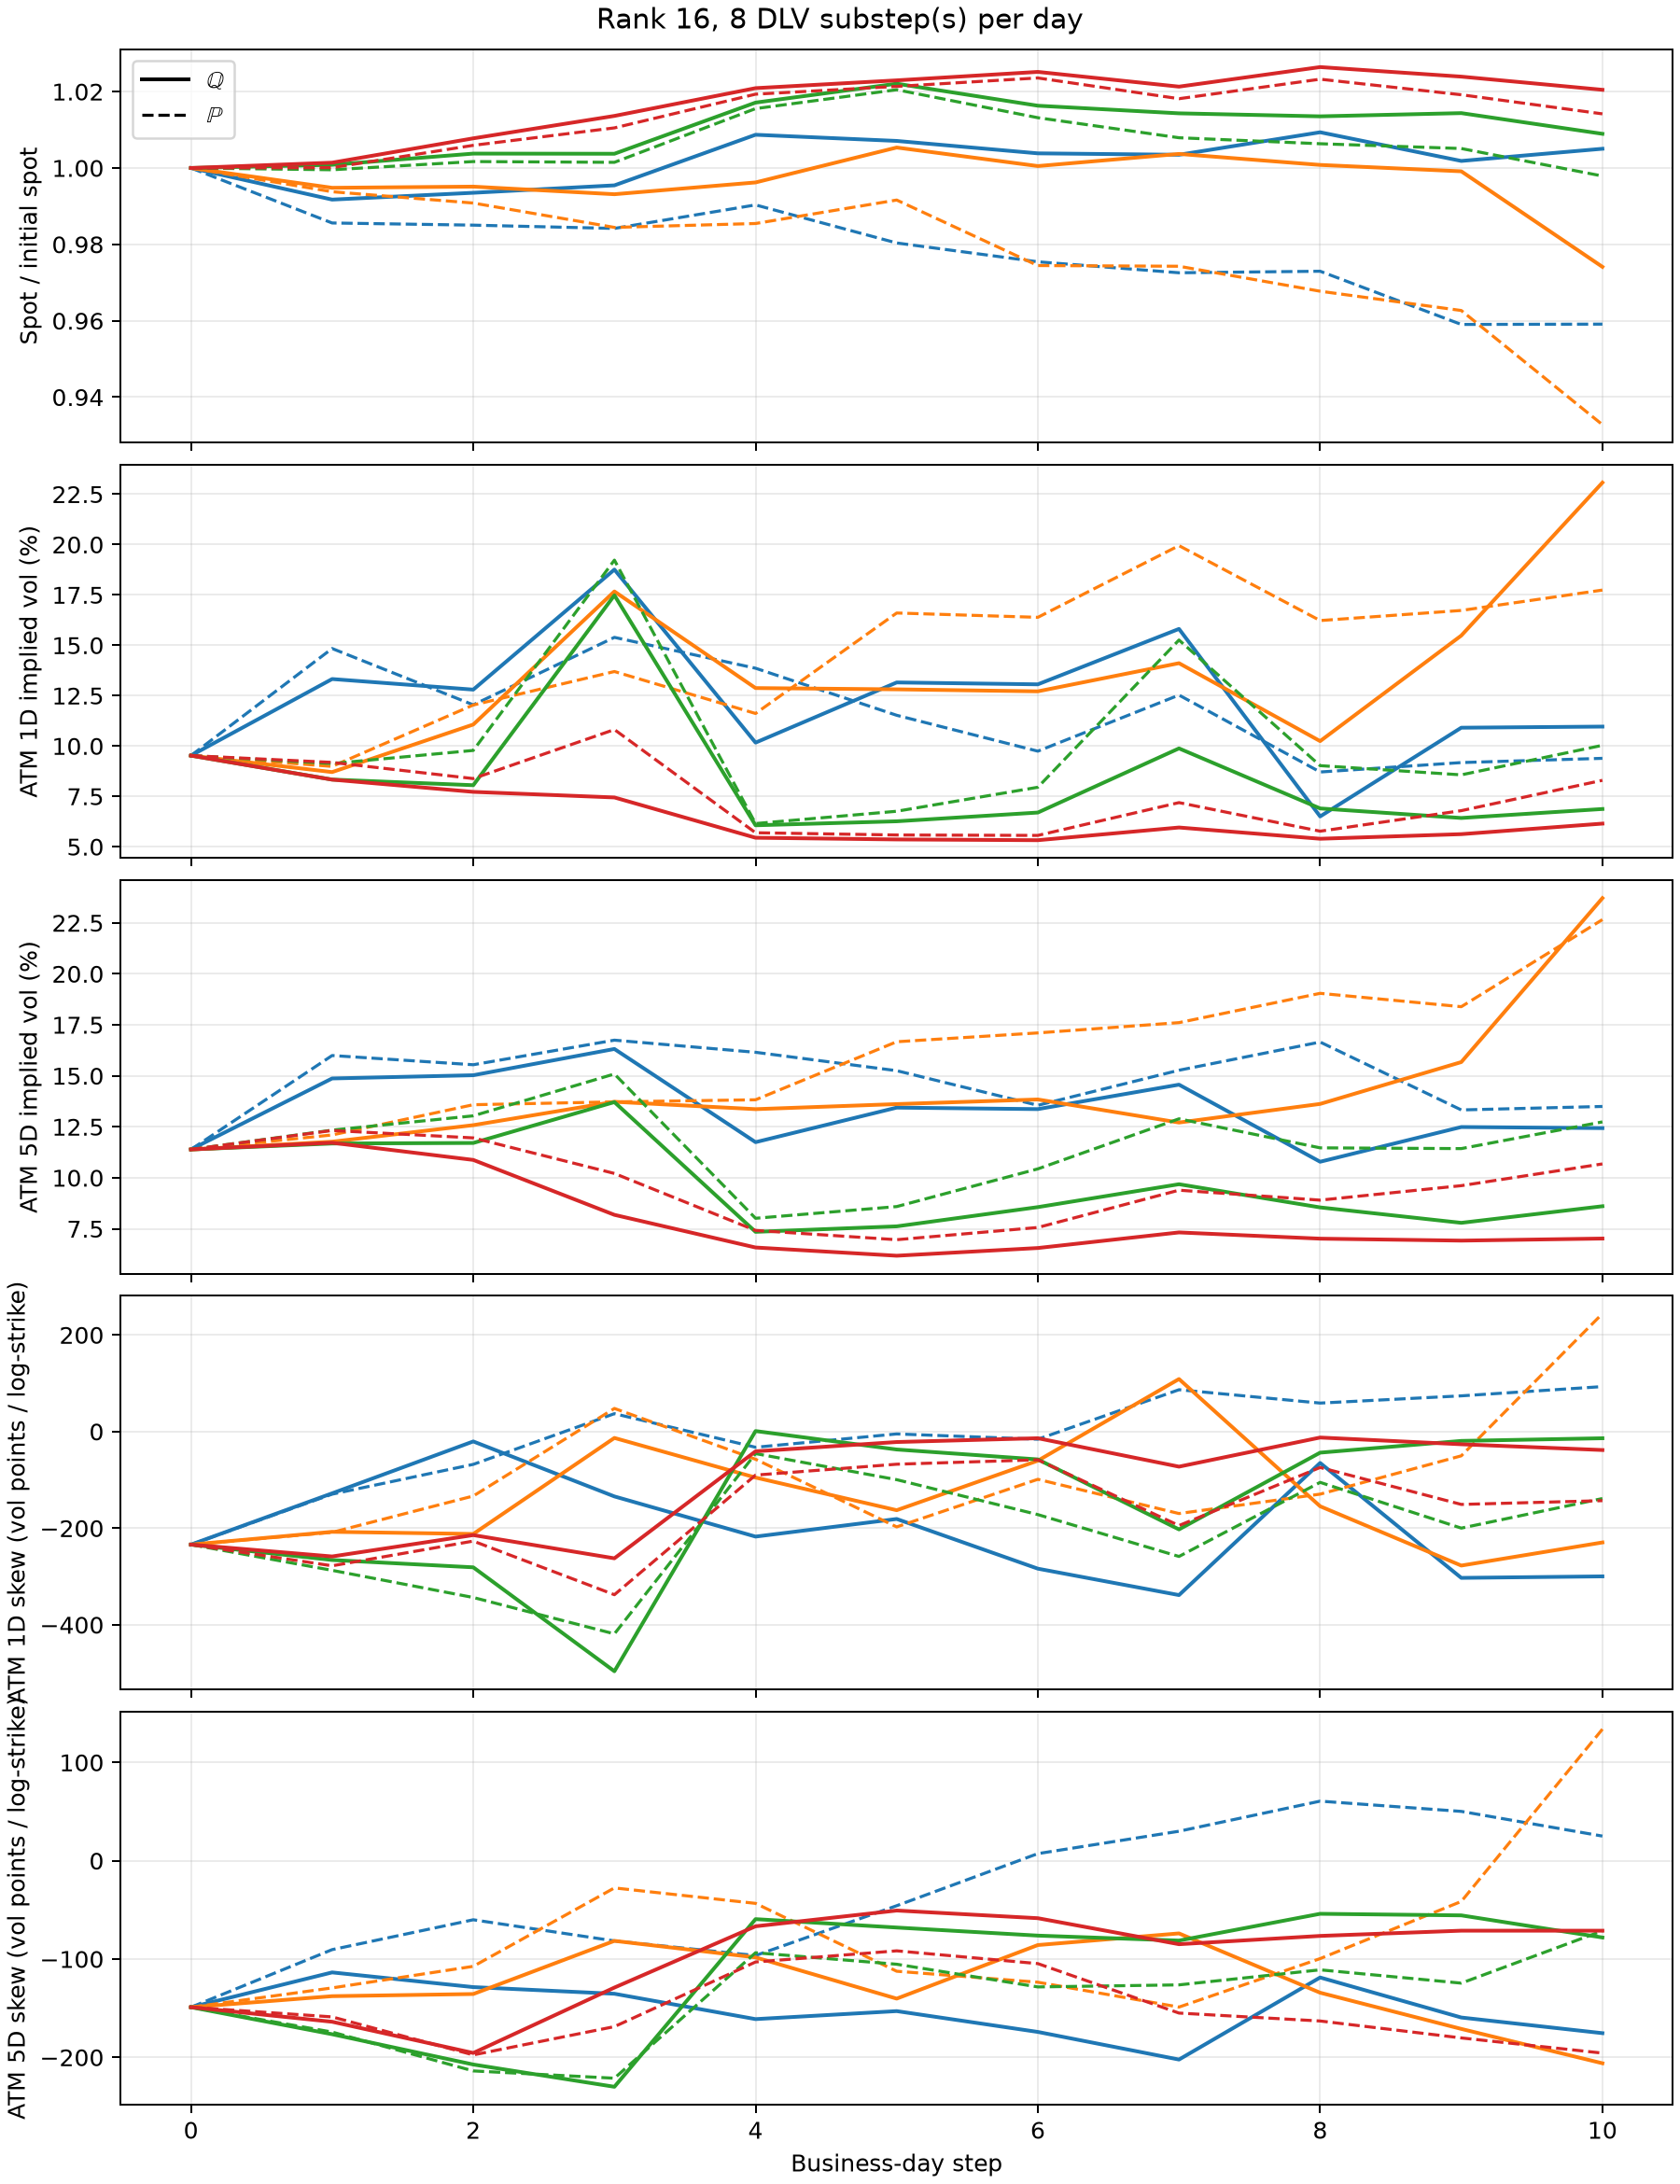
\includegraphics[height=0.88\textheight]
    {figures/front_spot/paths_rank16_eight_step.png}
  \caption{Matched $\PP/\Q$ paths for Model~D: rank 16 with eight Brownian
  substeps per day.}
  \label{fig:numerics-best-paths}
\end{figure}

\subsection{PCA Summary}
\label{app:dlv-factor-figures}

The remaining figures visualize the factor systems estimated in
Section~\ref{sec:estimation-vol-of-vol}.  Figure~\ref{fig:numerics-baseline-iv-3d}
is the baseline risk-neutral implied-volatility surface used for all factor
illustrations.


\begin{figure}[H]
  \centering
  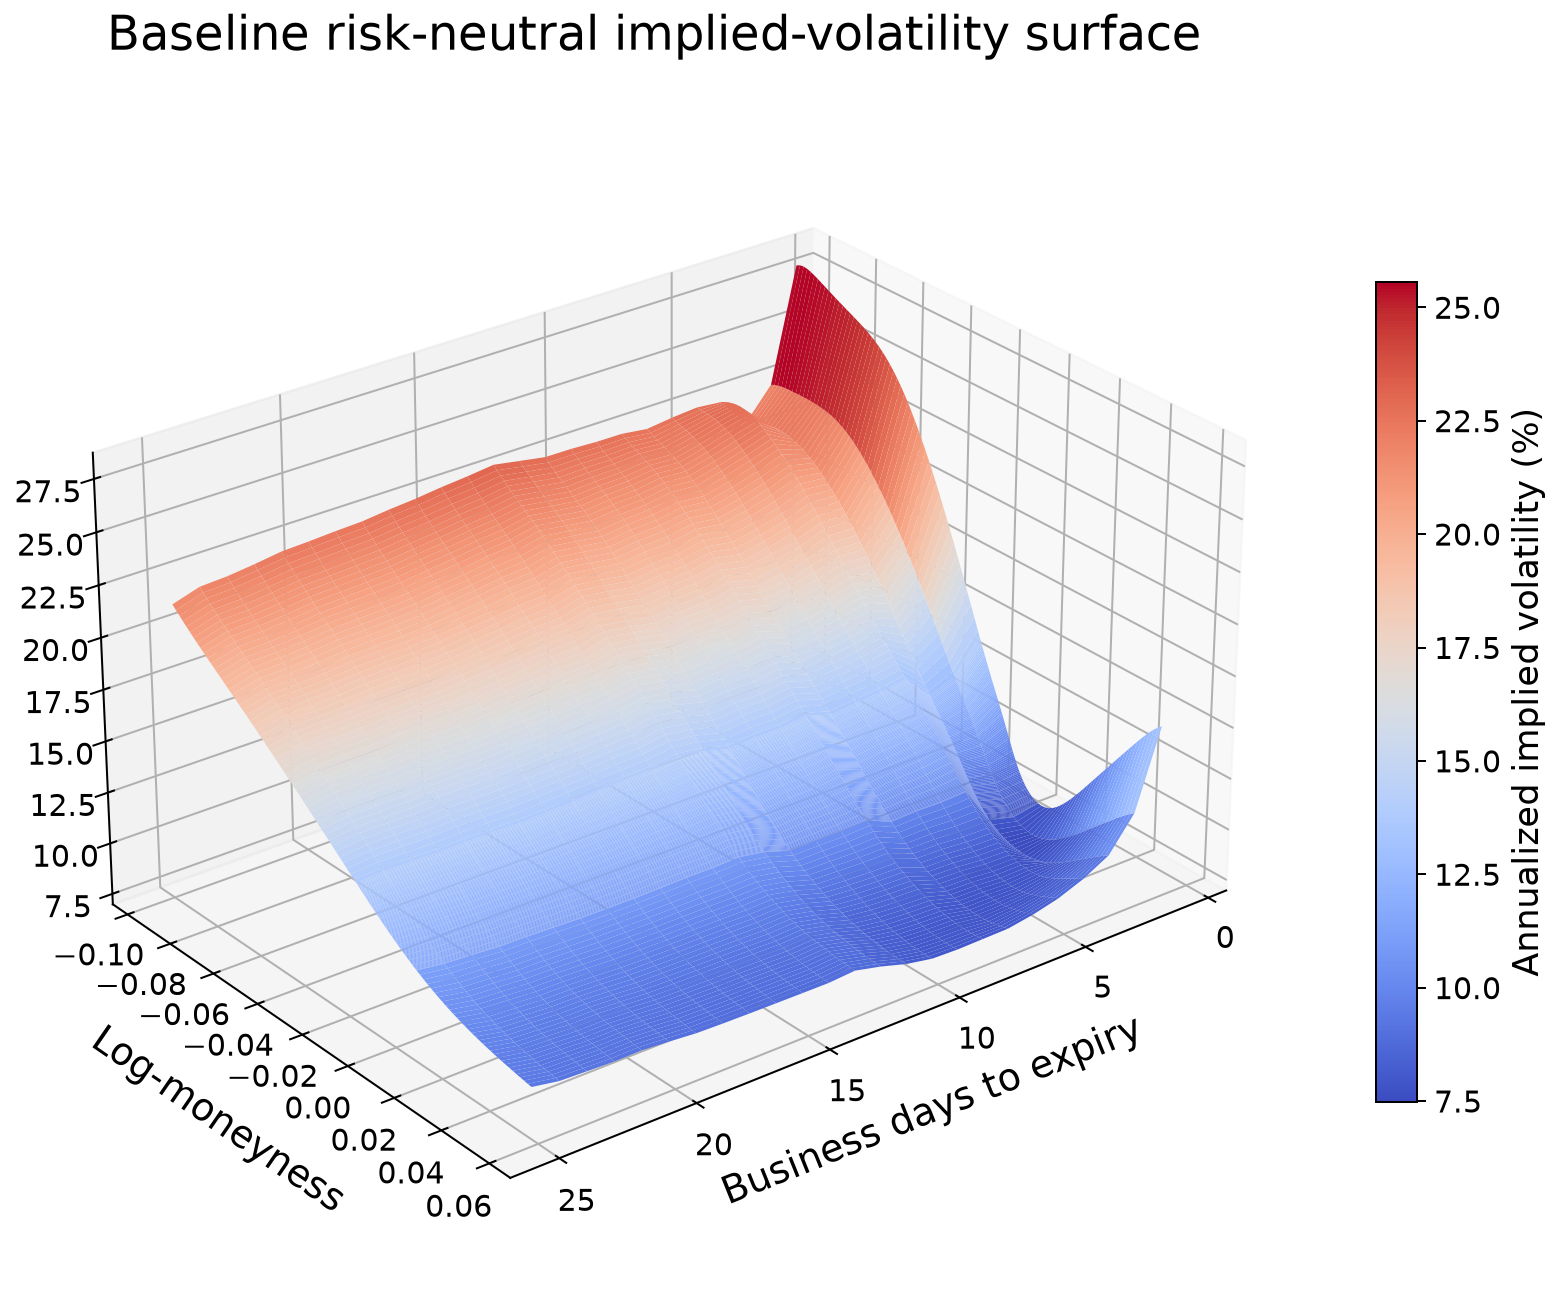
\includegraphics[width=0.72\textwidth]
    {figures/front_spot/baseline_implied_volatility_3d.png}
  \caption{Baseline annualized implied volatility on the fitted
  log-moneyness and business-days-to-expiry grid.}
  \label{fig:numerics-baseline-iv-3d}
\end{figure}

Figure~\ref{fig:numerics-factor-power} reports individual and cumulative PCA
power.  The experiments retain either eight or 16 factors; the first rank
above 90\% is 26.

\begin{figure}[H]
  \centering
  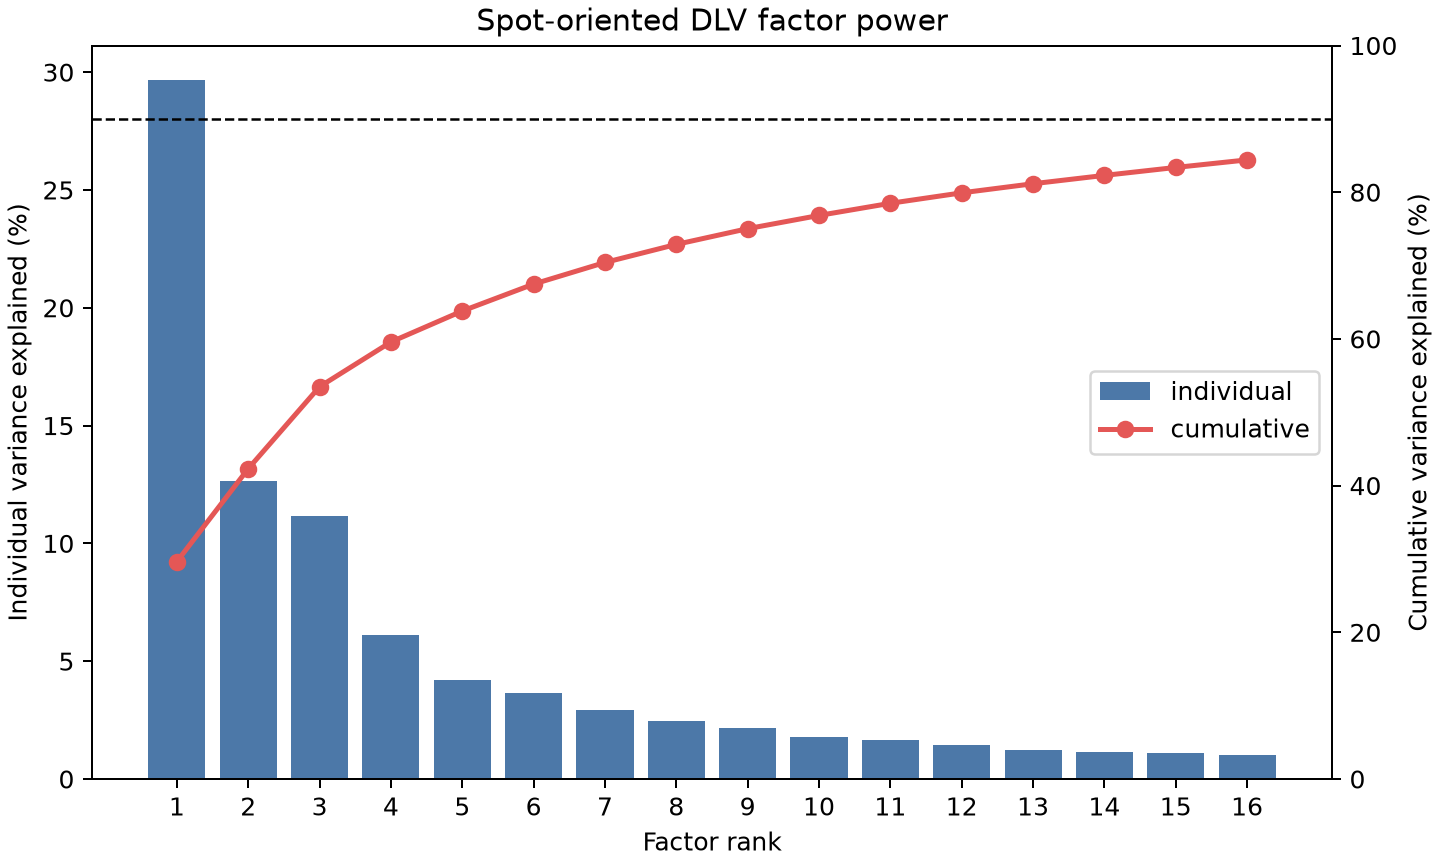
\includegraphics[width=0.88\textwidth]
    {figures/front_spot/pca_explained_variance.png}
  \caption{Individual and cumulative variance explained by the spot-oriented
  DLV factor system.  The vertical line is the rank-16 model cap; 26 factors
  are required to exceed 90\%.}
  \label{fig:numerics-factor-power}
\end{figure}

The rank-16 fit appends PCs 9--16 to the rank-8 fit.  A one-standard-deviation
shock is the diffusion-only log-DLV displacement
$\pm\xi_f\sqrt{1/252}$.  The figures display its central implied-volatility
response
\begin{equation}
  \label{eq:numerics-iv-factor-shock}
  \frac12\left[
    \sigma_{\mathrm{imp}}(\log\Sigma+\xi_f/\sqrt{252})
    -\sigma_{\mathrm{imp}}(\log\Sigma-\xi_f/\sqrt{252})
  \right].
\end{equation}
These shock directions are the same under $\PP$ and $\Q$: an equivalent
measure change alters drift, not diffusion.  Each panel deliberately retains
its own vertical scale.

\begin{figure}[H]
  \centering
  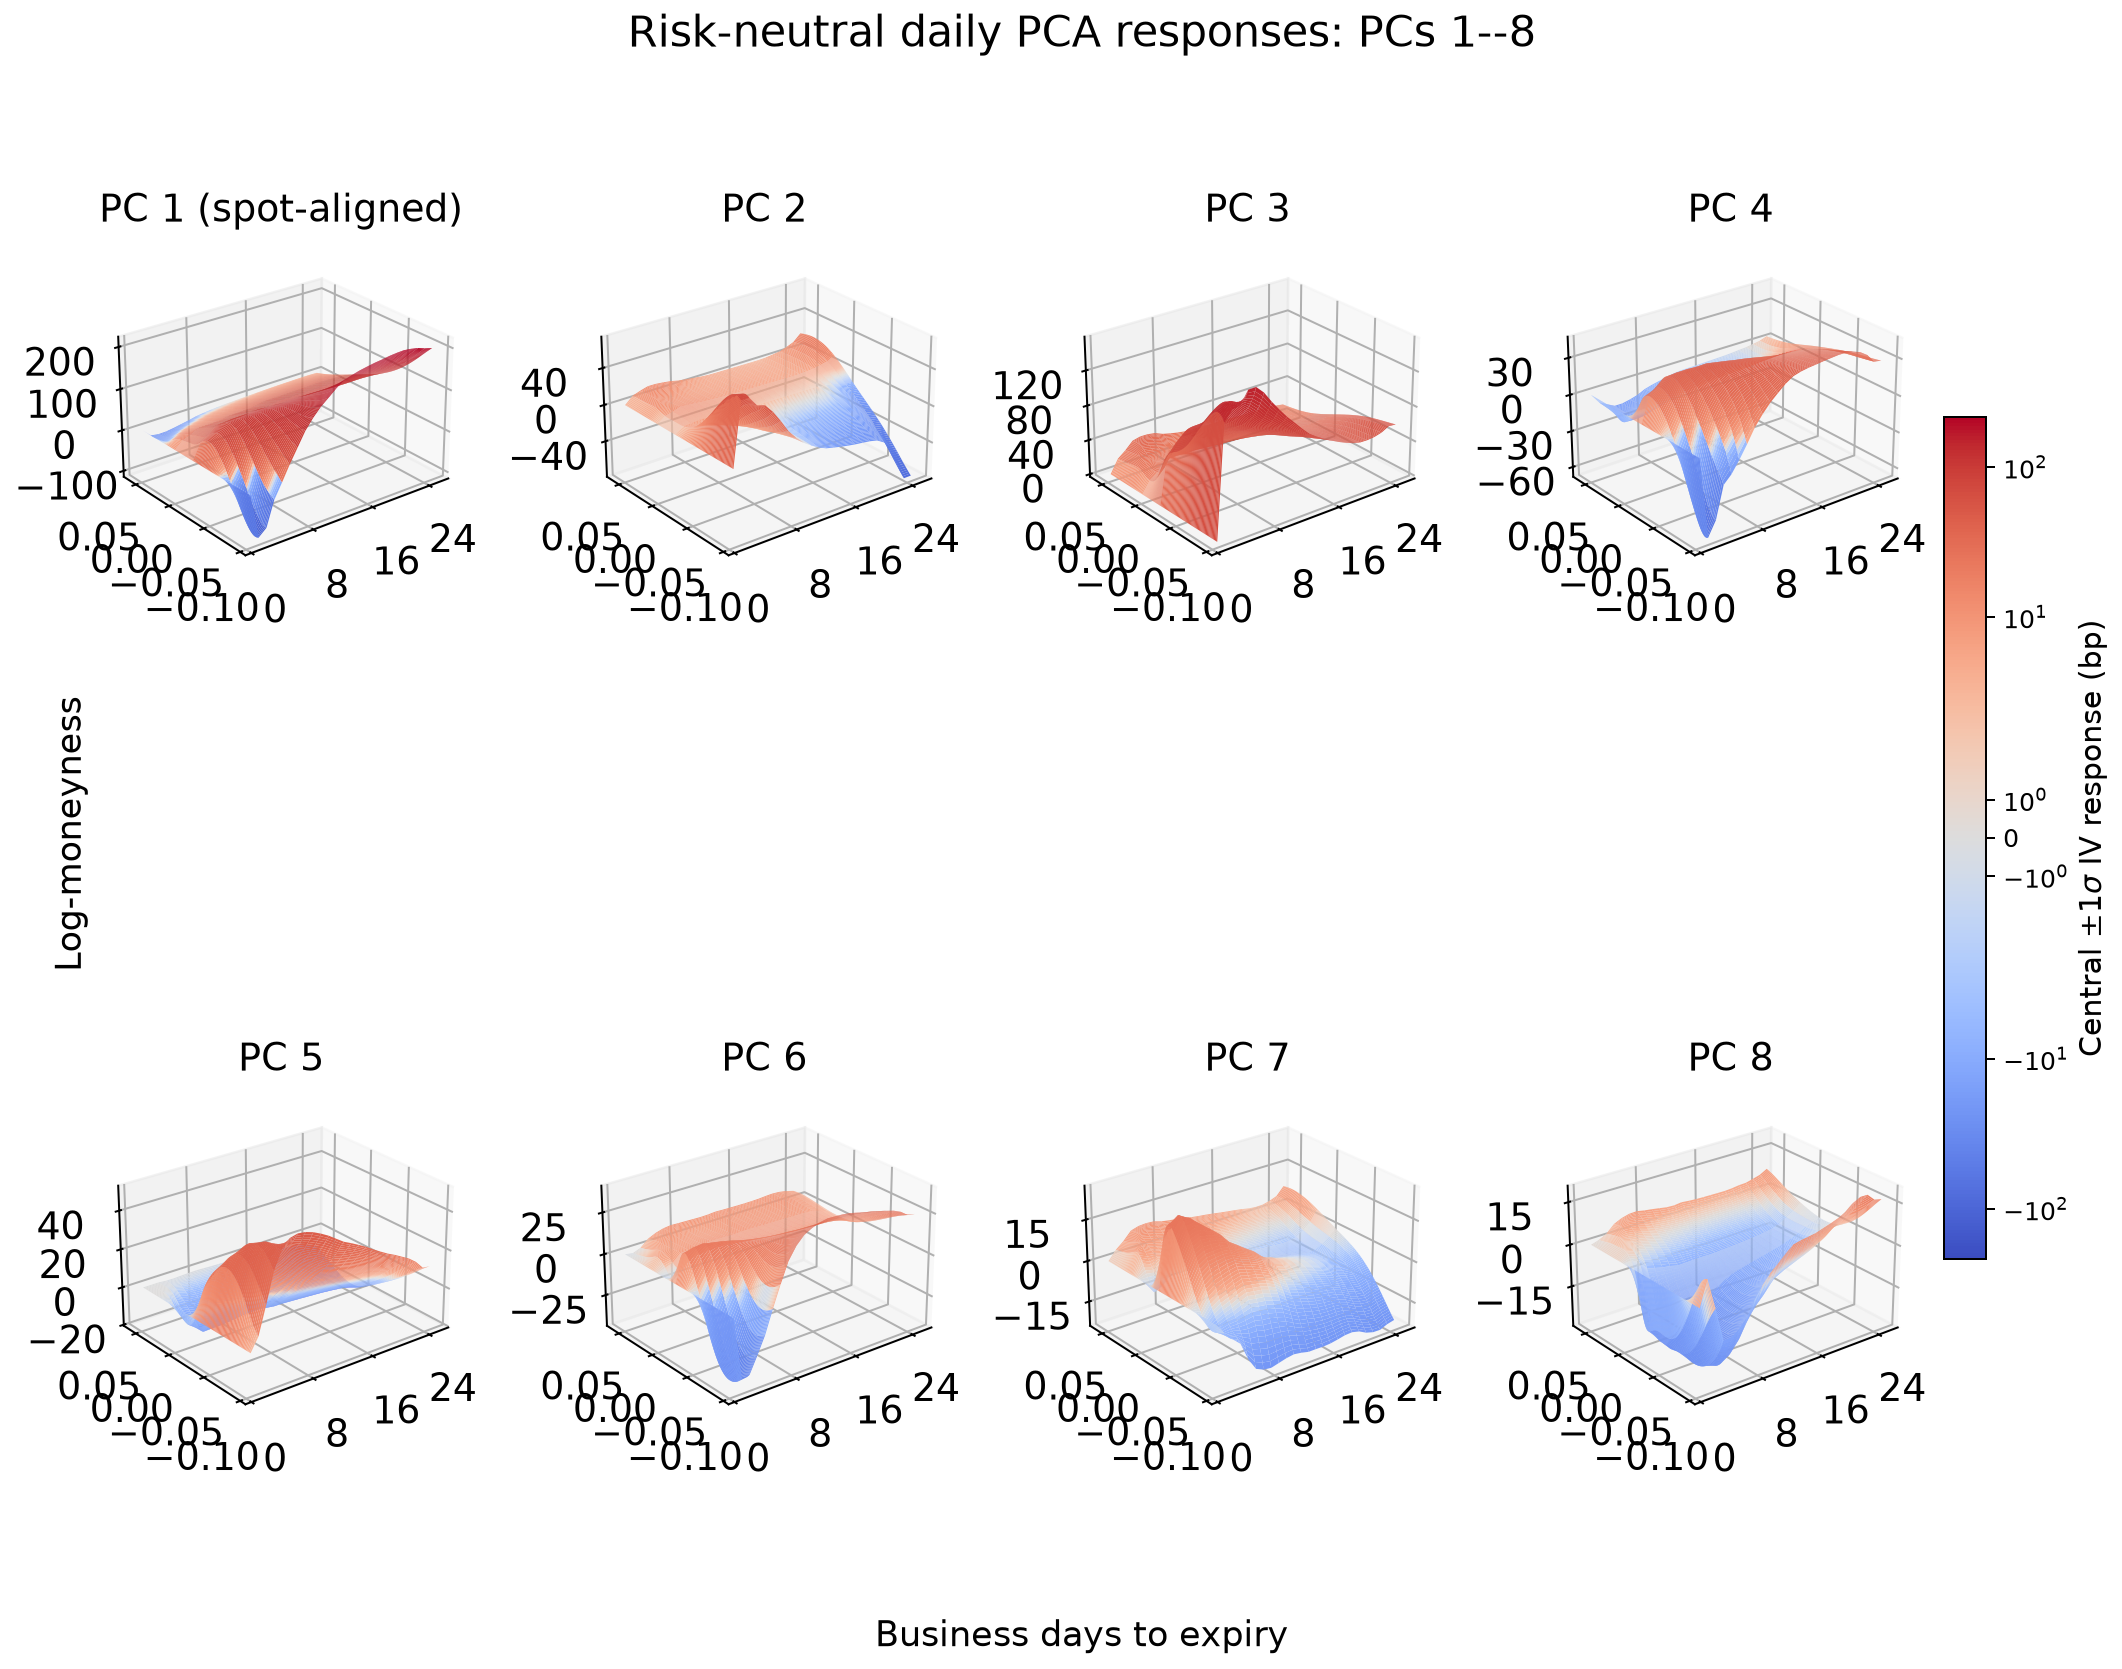
\includegraphics[width=\textwidth]
    {figures/front_spot/pca_factor_responses_3d_pc1_8.png}
  \caption{Risk-neutral one-standard-deviation implied-volatility responses
  for PCs 1--8.  PC~1 is aligned to the front-spot score.}
  \label{fig:numerics-pc1-8}
\end{figure}

\begin{figure}[H]
  \centering
  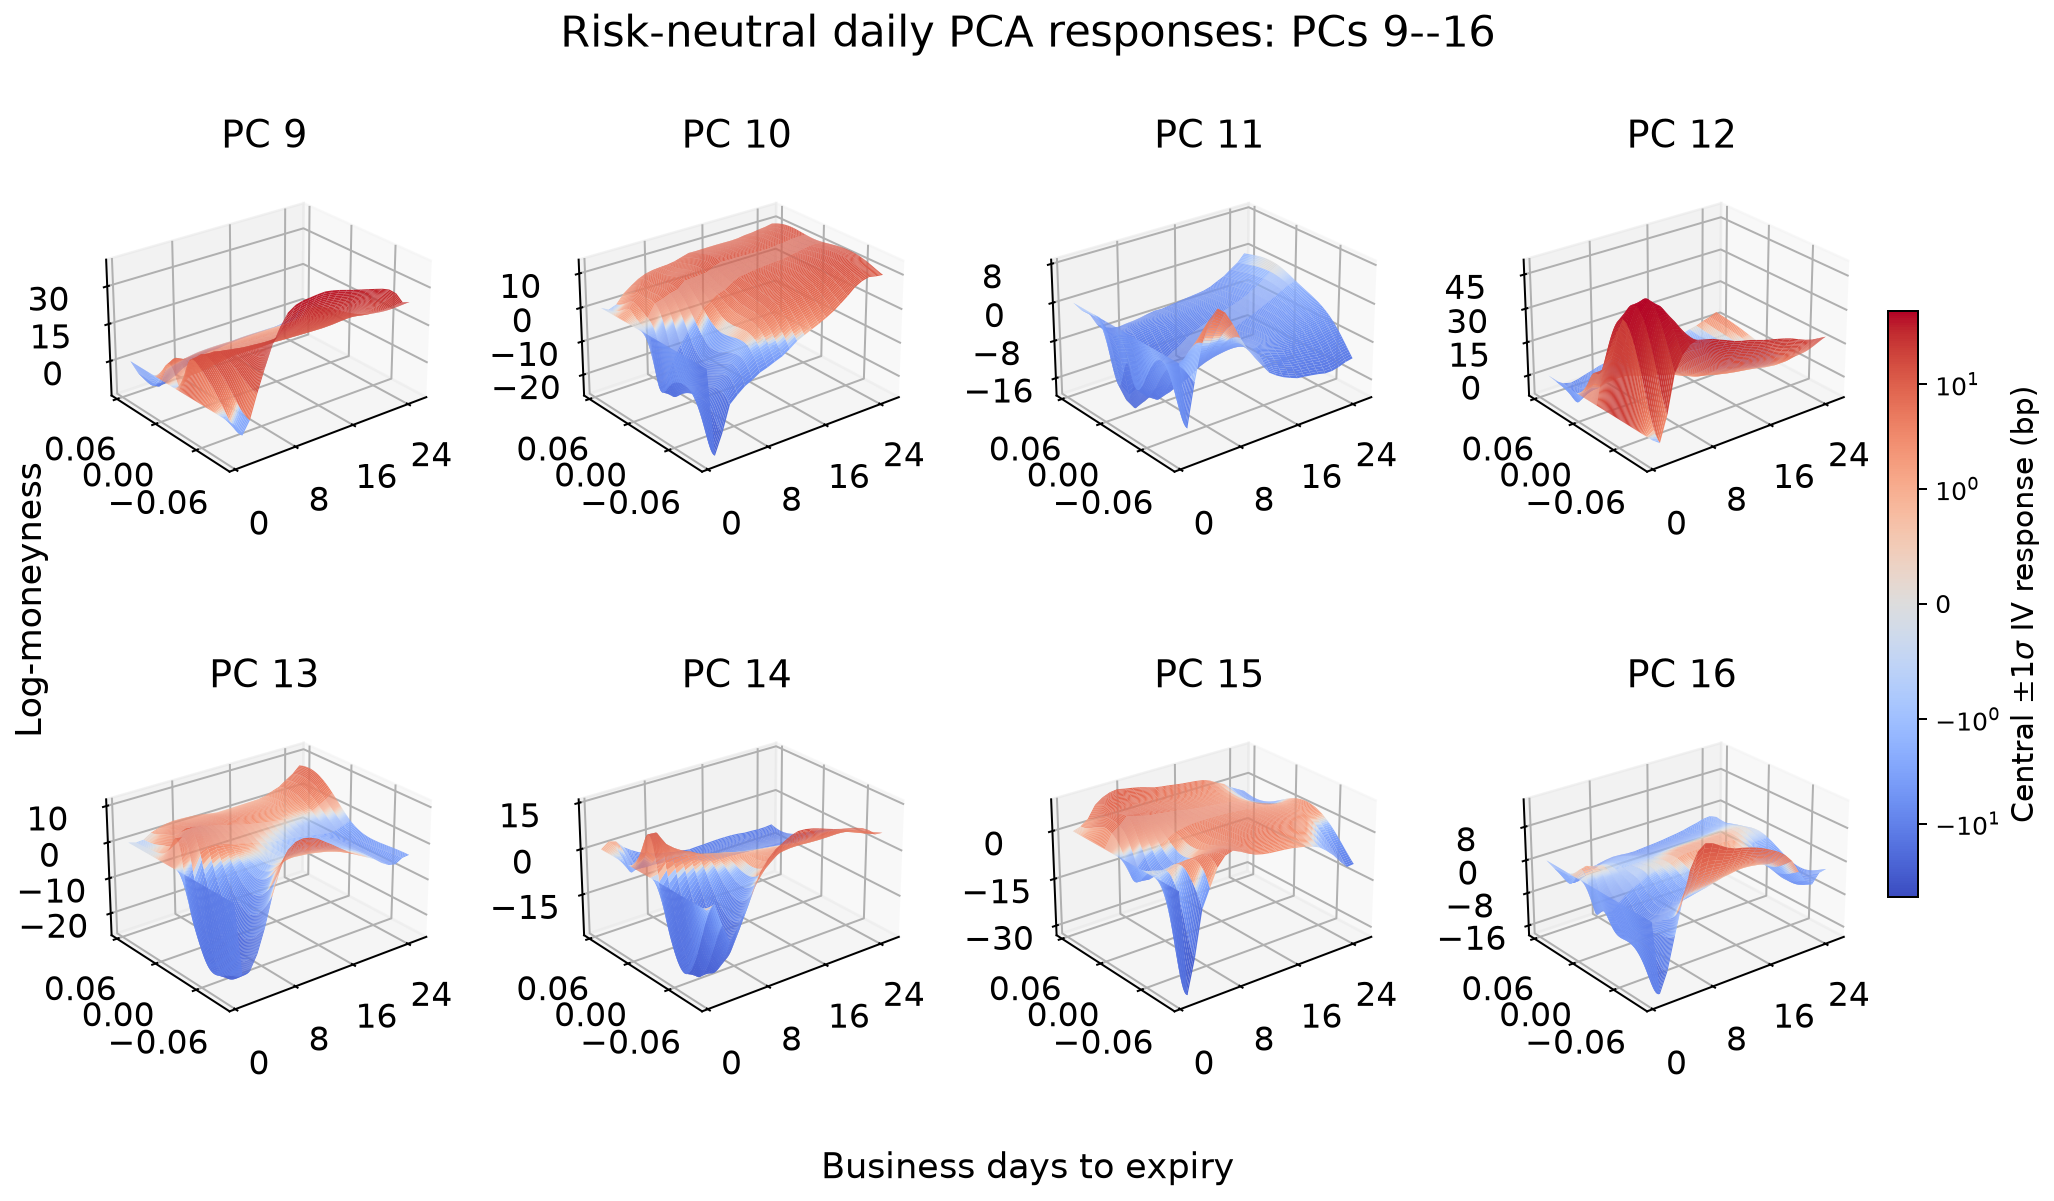
\includegraphics[width=\textwidth]
    {figures/front_spot/pca_factor_responses_3d_pc9_16.png}
  \caption{The additional one-standard-deviation implied-volatility responses,
  PCs 9--16, in the nested rank-16 model.}
  \label{fig:numerics-pc9-16}
\end{figure}

% !TEX root = main2.tex
\section{Market-data and calibration pipeline}
\label{app:market-pipeline}

This appendix records the data and numerical pipeline behind
Section~\ref{sec:estimation}. It follows the broader SPX pipeline described in
\cite{DYSANOS2026}, restricted here to the short-dated fixed-expiry SANOS
experiment. The complete transformation is
\[
\begin{aligned}
\text{raw IvyDB quotes}
&\longrightarrow \text{daily cleaning and parity-forward enrichment}\\
&\longrightarrow \text{arbitrage-free SANOS eligibility surface}\\
&\longrightarrow \text{European short-horizon quote selection}\\
&\longrightarrow \text{daily 25-by-200 calibration tensor}\\
&\longrightarrow \text{direct or affine end-to-end fit}.
\end{aligned}
\]

\subsection{Raw data and cleaning}
\label{app:pipeline-raw}

The source is OptionMetrics IvyDB US data accessed through WRDS. For each
eligible SPX market date we load the index level and previous index level,
option strikes and calendar expiries, call and put bid and ask quotes, volume,
open interest, AM/PM settlement flags, and the zero curve. The retained sample
runs from 3 January 2022 through 29 August 2025 and contains 891 valid full-day
NYSE sessions.

The raw cleaning step removes known bad ticker--date observations, missing or
invalid quotes, invalid settlement flags, same-day expiries, irregular
expiries, and quotes whose bid does not exceed $0.011$. Business days and year
fractions to expiry are then computed; an AM-settled expiry is treated as
$0.2$ of a business day earlier than its corresponding PM expiry.

For each expiry we recompute the forward from put--call parity rather than use
the delayed IvyDB forward table. With discount factor $D$, define the
discounted-forward bounds at a strike $K$ by
\[
  G^{\mathrm{ask}}(K)=C^{\mathrm{ask}}(K)-P^{\mathrm{bid}}(K)+DK,
  \qquad
  G^{\mathrm{bid}}(K)=C^{\mathrm{bid}}(K)-P^{\mathrm{ask}}(K)+DK.
\]
Their midpoint is averaged across strikes with inverse-spread weights,
\[
  \widehat G
  =\frac{\sum_K w_K\,[G^{\mathrm{ask}}(K)+G^{\mathrm{bid}}(K)]/2}
         {\sum_K w_K},
  \qquad
  w_K=\frac1{\max\{G^{\mathrm{ask}}(K)-G^{\mathrm{bid}}(K),10^{-3}\}}.
\]
The resulting forward is used to construct the tightest call-equivalent quote,
forward-normalized strikes and prices, implied volatilities, and Greeks. An
expiry must contain at least ten strikes with a traded call or put and at least
four strikes with both sides traded. The normalized spread must exceed
$10^{-6}$ and retained implied volatilities must lie between $0.01$ and $5$.

\subsection{Static preprocessing and quote selection}
\label{app:pipeline-static}

Before applying the model-specific horizon, the pipeline retains quotes with
vega per unit total volatility of at least $10^{-3}$, log volume and log open
interest of at least one, and at least ten surviving options per expiry. The
nominal per-day quote cap is 100,000 and is therefore non-binding here.

For data-quality control and to construct a stable ATM curve, every daily book
is passed through the linear SANOS preprocessing of \cite{SANOS2026}. The
strike grid is extended, each expiry is fitted inside the quoted bid--ask
intervals, negligible-density redundant strikes are removed, and the joint
surface fit enforces both butterfly and calendar-spread constraints. The
smoothness parameter is $0.25$. Expiries and strikes for which this
arbitrage-free auxiliary fit is unavailable are not passed to the final
calibration.

This auxiliary SANOS surface determines eligibility, the ATM term structure,
and the floating model support. It is not the calibration target: the JAX fits
in Section~\ref{sec:estimation-fit} use the original retained call and put
bid--ask intervals. No linear-programming state or fitted midpoint is supplied
as a target.

The final selection keeps European quotes no farther than 25 business days
from the observation date, excludes the $0.2$-business-day slice, and retains
the standardized log-moneyness interval $[-2.5,1.5]$. This leaves 2,192,458
quotes, between 1,590 and 5,096 per date.

\subsection{Daily calibration tensor}
\label{app:pipeline-tensor}

The model expiry grid is
\[
  T_j=\frac{j}{252},\qquad j=1,\ldots,25.
\]
For each date, 100 interior-strike candidates are generated from the front
ATM scale and 100 from the 25-day ATM scale. They are merged with a minimum
log-spacing safeguard to form one 200-node support shared across all model
expiries on that date. The support floats from date to date. Two boundary
nodes, equal to one half of the lowest inner strike and one and a half times
the highest inner strike, complete the 202-node density grid.

Each retained market quote stores its call/put flag, normalized strike, bid,
ask, midpoint, business days to expiry, adjacent model-expiry indices, and
linear interpolation weight. The contemporaneous SPX level is retained as a
reference spot. The immutable calibration tensor pads each date to a multiple
of 128 quotes and carries a Boolean mask, so padding never contributes to the
objective.

At valuation time the DLV recursion produces the 25 discrete densities. The
fixed 5\% Black factor convolves each discrete density into a smooth call-price
curve, and the two adjacent expiry curves are linearly interpolated to the
market quote's exact expiry. Puts follow from put--call parity.

\subsection{Optimization and retained artifacts}
\label{app:pipeline-optimization}

The direct and affine parameterizations are those in
Section~\ref{sec:estimation-fit}. Direct states are initialized from the
date-specific ATM term structure and are constant across strike at
initialization. Affine means use the average of these initial states; codes and
loadings receive small centered Gaussian initial values. DLV squared is bounded
between $10^{-4}$ and $9$, with a differentiable barrier near the upper bound.

The loss in \eqref{eq:estimation-quote-objective} is differentiated over every
retained quote. Quote blocks of size 128 are used only to limit accelerator
memory: their gradients are summed before each Adam update, so this is an exact
full-sample gradient rather than stochastic minibatching. Each fit uses 300
initial epochs with a cosine learning-rate schedule from $2\times10^{-2}$ to
$10^{-3}$, followed by a 700-epoch continuation from $5\times10^{-3}$ to
$5\times10^{-5}$. Checkpoints store either all daily direct states or the
affine mean, loadings, and daily codes. The retained reports recompute every
quote from the final checkpoint and produce the statistics in
Table~\ref{tab:numerics-static-market-fit}.


\bibliographystyle{alpha}
\bibliography{refs}

\end{document}
